% Festlegung des allgemeinen Dokumentenformats
\documentclass[a4paper,12pt]{article}

% Schrift
\usepackage[T1]{fontenc}
\usepackage{lmodern}
\usepackage[utf8]{inputenc}
\usepackage[ngerman]{babel}

% Bilder
\usepackage{graphicx}
\usepackage{float}
\graphicspath{{./assets/img}}

% Variablen
% Variablen
\newcommand{\titleDocument}{Masterarbeit}
\newcommand{\subjectDocument}{StudyMap: Konzeption und Evaluierung eines
innovativen Studiengangfinders am Beispiel der OTH-Regensburg}
\newcommand*{\bildquelle}{
  \footnotesize Quelle:
}
\newcommand{\code}[1]{\noindent\ignorespaces\texttt{#1}}

% Code
\usepackage{listings}
\usepackage{color}

\definecolor{black}{rgb}{0,0,0}
\definecolor{dkgreen}{rgb}{0,0.6,0}
\definecolor{gray}{rgb}{0.5,0.5,0.5}
\definecolor{mauve}{rgb}{0.58,0,0.82}

\lstset{literate=%
    {Ö}{{\"O}}1
    {Ä}{{\"A}}1
    {Ü}{{\"U}}1
    {ß}{{\ss}}1
    {ü}{{\"u}}1
    {ä}{{\"a}}1
    {ö}{{\"o}}1
    {~}{{\textasciitilde}}1
}

\lstdefinestyle{Bash} {
  frame=single,
  language=Bash,
  aboveskip=3mm,
  belowskip=3mm,
  showstringspaces=false,
  columns=flexible,
  basicstyle={\small\ttfamily},
  numbers=none,
  numberstyle=\tiny\color{black},
  keywordstyle=\color{black},
  commentstyle=\color{black},
  stringstyle=\color{black},
  breaklines=true,
  breakatwhitespace=true,
  tabsize=3
}

\lstset{emph={\$},emphstyle=\textbf}

\lstdefinestyle{Python} {
  frame=single,
  language=Bash,
  aboveskip=3mm,
  belowskip=3mm,
  showstringspaces=false,
  columns=flexible,
  basicstyle={\small\ttfamily},
  numbers=left,
  numberstyle=\tiny\color{mauve},
  keywordstyle=\color{mauve},
  commentstyle=\color{dkgreen},
  stringstyle=\color{dkgreen},
  breaklines=true,
  breakatwhitespace=true,
  tabsize=2
}

% mehrseitige Tabellen ermöglichen
\usepackage{longtable}
\usepackage{diagbox}

% Packet für Seitenrandabstände und Einstellung für Seitenränder
\usepackage{geometry}
% Internet
%\geometry{left=3.5cm, right=2.5cm, top=2.5cm, bottom=2cm}
% Kern
\geometry{a4paper, top=27mm, left=20mm, right=20mm, bottom=35mm, headsep=10mm,
footskip=12mm}

% bricht lange URLs "schön" um
\usepackage[hyphens,obeyspaces,spaces]{url}

% Festlegung Art der Zitierung
\usepackage{csquotes}
\usepackage[style=apa, backend=biber]{biblatex}
\addbibresource{assets/literatur.bib}

% Abstand zwischen Absätze
\setlength{\parindent}{2em}
\setlength{\parskip}{1em}

% Paket für Zeilenabstand
\usepackage{setspace}
\onehalfspacing
% Kern:
% \setstretch{1.15}

% für Bildbezeichner
\usepackage{capt-of}

% für Stichwortverzeichnis
\usepackage{makeidx}

% für Abkürzungsverzeichnis
\usepackage{acronym}

% Für Phantomsection
\usepackage{hyperref}

% Für Tabellen
\usepackage{tabularx}

% Konfiguriere das Inhaltsverzeichnis
\usepackage{tocbasic}

% Anhang: PDF einfügen
\usepackage{pdfpages}

% subsubsubsection durch paragraph
\usepackage{titlesec}
\setcounter{secnumdepth}{4}
\titleformat{\paragraph}
{\normalfont\normalsize\bfseries}{\theparagraph}{1em}{}
\titlespacing*{\paragraph}
{0pt}{3.25ex plus 1ex minus .2ex}{1.5ex plus .2ex}
% Kern:
\titlespacing{\section}{0pt}{12pt plus 4pt minus 2pt}{8pt plus 2pt minus 2pt}
\titlespacing{\subsection}{0pt}{12pt plus 4pt minus 2pt}{6pt plus 2pt minus 2pt}
\titlespacing{\subsubsection}{0pt}{12pt plus 4pt minus 2pt}{4pt plus 2pt minus 2pt}

% \autoref: Subsubsection umbenennen
\addto\extrasngerman{
    \def\subsubsectionautorefname{Unterabschnitt}
}

% Titel
\title{Bachelorarbeit}

% Autor
\author{Andreas Huber}

% Datum
\date{\today}

%
% Start
% des
% Dokuments
%
\begin{document}

% Titelseite
\thispagestyle{empty}

\begin{figure}[t]
 \centering
 
\includegraphics[width=0.4\textwidth]{assets/oth/logo}
\end{figure}

\begin{verbatim}
\end{verbatim}

\begin{center}
    \Large{Ostbayerische Technische Hochschule Regensburg} \\
    \Large{Fakultät für Informatik und Mathematik}
\end{center}

\begin{verbatim}
\end{verbatim}

\begin{center}
    \doublespacing
    \textbf{\huge{\titleDocument}}\\

    \onehalfspacing

    \begin{center}
        Zur Erlangung des akademischen Grades \\ Master of Science (M. Sc.)
    \end{center}

    \begin{verbatim}
    \end{verbatim}

    \begin{doublespace}
        \textbf{\Large{{~\subjectDocument}}}
    \end{doublespace}
\end{center}

\begin{verbatim}
\end{verbatim}

\begin{verbatim}
\end{verbatim}

\begin{flushleft}
    \begin{tabularx}{\linewidth}{@{}>{\bfseries}l@{\hspace{.9em}}X@{}}
        \textbf{Vorgelegt von:} & Andreas Huber <andreas.huber@st.oth-regensburg.de> \\
        \textbf{Matrikelnummer:}& 3370380 \\
        \textbf{Studiengang:}   & Master Informatik (Schwerp. Software Engineering) \\
                                & \\
        \textbf{Erstgutachter:} & Prof. Dr. Markus Heckner \\
        \textbf{Zweitgutachter:}& Prof. Dr. Daniel Jobst \\
                                & \\
        \textbf{Abgabefrist:}   & 20. März 2024 \\
    \end{tabularx}
\end{flushleft}
\newpage

% Einverständniserklärung
\thispagestyle{empty}
\section*{Erklärung zur Masterarbeit}

\bigskip
\bigskip 
\bigskip 

\begin{enumerate}
    \item Mir ist bekannt, dass dieses Exemplar der Abschlussarbeit als Prüfungsleistung in das Eigentum der Ostbayerischen Technischen Hochschule Regensburg übergeht.
    \item Ich erkläre hiermit, dass ich diese Abschlussarbeit selbständig verfasst, noch nicht anderweitig für Prüfungszwecke vorgelegt, keine anderen als die angegebenen Quellen und Hilfsmittel benutzt sowie wörtliche und sinngemäße Zitate als solche gekennzeichnet habe.
\end{enumerate}

\bigskip 
\bigskip 
\bigskip 

\noindent Regensburg, den \today

\bigskip 
\bigskip

\noindent\line(1,0){200}
\newline
\noindent Andreas Huber
\newpage

% Römische Nummerierung
\pagenumbering{Roman}

% Inhaltsverzeichnis
\tableofcontents

% Abbildungsverzeichnis
\newpage
\phantomsection
\addcontentsline{toc}{section}{Abbildungsverzeichnis}
\renewcommand\refname{Abbildungsverzeichnis}

\listoffigures

% Tabellenverzeichnis
\newpage
\phantomsection
\addcontentsline{toc}{section}{Tabellenverzeichnis}
\renewcommand\refname{Tabellenverzeichnis}

\listoftables

% Abkürzungsverzeichnis
\newpage
\phantomsection
\section*{Abkürzungsverzeichnis}
\addcontentsline{toc}{section}{Abkürzungsverzeichnis}

\begin{acronym}[Bash]
    % \acro{bash}[Bash]{Bourne-again shell}
    % \acro{ide}[IDE]{Integrated Development Environment}
    % \acro{ldap}[LDAP]{Lightweight Directory Access Protocol}
    % \acro{lms}[LMS]{Learning Management System}
    % \acro{oth}[OTH]{Ostbayerische Technische Hochschule}
    % \acro{sd}[SD]{Standardabweichung}
\end{acronym}

% Arabische Seitennummerierung ab hier
\newpage
\pagenumbering{arabic}

% Einleitung
\section{Einleitung}\label{einleitung}
\subsection{Einleitung und Motivation}\label{einleitung-und-motivation}
Die Wahl des richtigen Studiengangs ist ein wichtiger Schritt im Leben eines jeden angehenden Studierenden. Sie legt den Grundstein für die akademische und berufliche Entwicklung und beeinflusst den individuellen Bildungsweg maßgeblich. Angesichts der Vielfalt an verfügbaren Studiengängen stehen Studieninteressierte vor einer komplexen Entscheidung, die durch eine breite Palette von Inhalten,  Schwerpunkten und Karrierewegen geprägt ist. Diese Vielzahl an Informationen kann zu Unsicherheit und Verwirrung führen, wodurch nicht selten falsche Studienentscheidungen getroffen werden. \parencite{beckmann_verbesserung_2021}

Die vorliegende Masterarbeit greift dieses weit verbreitete Problem auf und stellt einen innovativen Ansatz zur Studienorientierung vor. Das Ziel ist es, eine benutzerfreundliche, automatisch generierte Infografik-basierte Plattform zu entwickeln, die Studieninteressierte dabei unterstützt, fundierte Entscheidungen über ihren zukünftigen Bildungsweg zu treffen. Die Anwendung namens StudyMap kombiniert moderne Datenanalyse, interaktive Benutzeroberflächen und nutzerzentriertes Design, um den Orientierungsprozess zu optimieren.

\subsection{Problemstellung/Zielsetzung}\label{problemstellung-zielsetzung}
Die derzeitige Studienorientierung wird oft durch eine Informationsflut und eine begrenzte Transparenz der verfügbaren Studiengänge behindert. Häufig kennen Studieninteressierte einen Studiengang oder eine ungefähre Richtung, in die sie gehen möchten. Um ähnliche Studiengänge oder alle Studiengänge in der gewünschten Richtung zu finden, fehlt oft der Überblick. \parencite{beckmann_verbesserung_2021} Diese Unsicherheit kann zu falschen Studienentscheidungen führen, die wiederum Studienabbrüche durch Motivationsmangel zur Folge haben \parencite{heublein_ursachen_2010}.

\noindent
Die spezifischen Ziele dieser Arbeit sind:
\begin{enumerate}
\item Entwicklung eines Konzepts für einen Studiengangsfinder auf Basis einer
interaktiven Infografik-basierten Benutzeroberfläche.
\item Implementierung und technische Umsetzung des entwickelten Systems am
Beispiel der Ostbayerischen Technischen Hochschule Regensburg (OTH-Regensburg).
\item Evaluation und Validierung eines Prototypen durch Tests mit potenziellen
Nutzern und Analyse der Ergebnisse.
\item Diskussion der Stärken und Schwächen des entwickelten Systems sowie der
möglichen Auswirkungen auf die Studienberatung.
\item Die Ergebnisse dieser Arbeit sollen dazu beitragen, die
Studienorientierung für Studieninteressierte zu erleichtern und ihnen bessere
Informationen und Orientierungshilfen zur Verfügung zu stellen.
\end{enumerate}

\subsection{Gliederung der Arbeit}
Die Arbeit beginnt nach der Einleitung mit dem theoretischen Hintergrund. Es werden bereits existierende Werkzeuge und Konzepte zur Studienorientierung beschrieben und die Theorie der Anwendung von interaktiven Systemen definiert.

Anschließend folgt das Kapitel \nameref{sec:methodik}, in dem zunächst verschiedene mögliche Algorithmen zur Darstellung aller Studiengänge besprochen werden. Daran anknüpfend werden die Datenquellen für den Studiengangsfinder hinsichtlich ihrer Herkunft bzw. Beschaffung diskutiert.

Das nächste Kapitel beschreibt das Konzept des innovativen Studiengangsfinders. Zunächst wird die Hochschule Regensburg als Fallbeispiel vorgestellt, einschließlich ihrer Herausforderungen und Ziele. Im Anschluss daran wird ein Konzept entwickelt, wie das Aussehen des Studiengangsfinders sein könnte und wie die Interaktivität gewährleistet werden kann. Außerdem wird in diesem Kapitel die Datenpflege und -sicherung behandelt. Dabei wird explizit auf die Datensicherung, die Trennung von Produktiv- und Testumgebung sowie auf eine Administrationsoberfläche eingegangen.

Das fünfte Kapitel behandelt den User-centered Design Prozess. Anhand von zwei Studien wird das Konzept evaluiert und verfeinert. Die erste Studie ist eine Mockup-Studie, in der das Designkonzept des Studiengangsfinders diskutiert wird. Auf der Grundlage dieser Ergebnisse wird ein Prototyp entwickelt, mit dem eine Prototypstudie mit 40 Personen, die sich für ein Studium interessieren, durchgeführt und diskutiert wird.

Nach Abschluss der Studien wird im Kapitel \nameref{sec:implementierung-und-deployment} zuerst die Auswahl der Technologien besprochen und daraufhin die Herausforderungen, die während der Implementierung entstanden sind. Schließlich werden die erläuterten Einzelkomponenten zusammengeführt und die daraus resultierende Softwarearchitektur, unterteilt in Frontend und Backend, erläutert. Der letzte Abschnitt dieses Kapitels befasst sich mit dem Software-Deployment. Es wird gezeigt, wie das Deployment abläuft, wie getestet werden kann und wie die Software letztendlich bereitgestellt wird.

Abschließend werden im letzten Kapitel die Ergebnisse und die wichtigsten Erkenntnisse zusammengefasst. Darüber hinaus wird ein Vergleich zu anderen Tools im Bereich der Studienorientierung gezogen und ein Ausblick gegeben. Im Rahmen dieses Ausblicks werden mögliche Erweiterungen und Anwendungen für die Zukunft diskutiert.
\newpage

% Theoretischer Hintergrund und vorhandene Studiengangsfinder-Konzepte
\section{Theoretischer Hintergrund und vorhandene Studiengangsfinder-Konzepte}
\subsection{Bisheriges Vorgehen bei der Studienorientierung}
% Wahl des Studiengangs PDF Seite 355
% Hochschulinformationstage wurden von MINT-Studierenden insgesamt häufig zur Studienentscheidung und Studienplanung genutzt (72 %).

% 1. Wichtigster Faktor Fach, 2. Ort o. Hochschultyp
% Oft kennen ein Fach, danach suchen sie einen Ort bzw. eine Hochschule
% Wenn sie dann auf die OTH Seite kommen, können sie nach der Kategorie suchen
% und dann ähnliche vielleicht noch besser passende Studiengänge finden
% Wichtigster Fachwahlgrund: Begabungen und pers. Neigungen
% Was Eltern, Verwandte u. Freunde sagen nur 0,1 %
% (Seite 67 von neuem PDF)
% 5 Typen schon Entscheidern, jeder entscheidet nach Pers. Neigung -> umso
% wichtiger ist es ihnen alle ähnlichen Studiengänge zu präsentieren!

Die Studienorientierung ist ein entscheidender Schritt im Bildungsweg eines
jeden Studieninteressierten und die Entscheidung für ein zukünftiges Studienfach
und eine Hochschule wird traditionell von verschiedenen Faktoren beeinflusst.
Eine umfassende Studie von CHE und EINSTIEG aus dem Jahr 2007 gibt Einblicke in
die Präferenzen und Entscheidungsmuster von Studieninteressierten.

Die Studie zeigt, dass für einen Großteil der Befragten (87,2 \%) die Wahl der
Hochschule und des Hochschulortes weniger relevant ist als das gewählte
Studienfach \parencite{einflussfaktoren}. Dies deutet darauf hin, dass das
persönliche Interesse an einem bestimmten Studienfach die Entscheidung stärker
beeinflusst als die geografische Lage oder der Ruf der Hochschule.

Ein weiteres wichtiges Ergebnis der Studie ist, dass 64,6 \% der Befragten ihr
Studienfach nach ihren Neigungen und Begabungen wählen
\parencite{einflussfaktoren}. Dies verdeutlicht, dass persönliche Neigungen und
individuelle Fähigkeiten die Studienentscheidung maßgeblich beeinflussen.

Die Erkenntnis, dass sich Studieninteressierte bei ihrer Studienfachwahl von
unterschiedlichen Motivationsfaktoren leiten lassen, führt zu der Vorstellung,
dass es verschiedene Entscheidungstypen gibt. Intrinsische Altruisten,
heimatgebundene Hedonisten, serviceorientierte Unabhängige und leistungsstarke
Karriereorientierte sind einige der identifizierten Gruppen, die jeweils
unterschiedliche Prioritäten bei der Fach-, Hochschul- und Ortswahl setzen.
Diese unterschiedlichen Entscheidungsmuster unterstreichen die Vielfalt
individueller Studienmotivationen. \parencite{einflussfaktoren}

In der Praxis bedeutet dies, dass Hochschulen wie die OTH-Regensburg darauf
achten müssen, ihre Studiengänge ansprechend und überzeugend zu präsentieren.
Gerade dann, wenn die Hochschule als mögliche Option in Betracht gezogen wird,
spielt die Möglichkeit, das gewünschte Fach entsprechend der individuellen
Interessen darzustellen, eine entscheidende Rolle.

Ein innovativer Studiengangsfinder, der Fächer inhaltlich kategorisiert und
ähnliche Studiengänge präsentiert, könnte hier eine wichtige Rolle spielen. Mit
einer solchen Lösung könnten Studieninteressierte effektiv über Alternativen
informiert werden, insbesondere wenn der ursprünglich angestrebte Studiengang
nicht verfügbar ist. Dies trägt dazu bei, dass die Hochschule potenzielle
Studierende auch dann überzeugen kann, wenn ihre erste Wahl nicht direkt
verfügbar ist, aber dennoch ähnliche, attraktive Alternativen bietet.


\subsection{Konzepte von Studiengangsfindern}
Die Historie der Studiengangsfinder zeigt eine dominierende Tendenz hin zu
umfragebasierten Konzepten. In diesem Zusammenhang werden Studierende durch
Umfragen zu ihren Interessen, Fähigkeiten und Präferenzen befragt, um auf dieser
Grundlage Studiengangsempfehlungen zu generieren.

Umfragebasierte Studiengangsfinder vertrauen auf die subjektiven Bewertungen
der Nutzer und versuchen, durch direkte Befragungen der Studierenden ihre
Präferenzen zu ermitteln. Die daraus resultierenden Empfehlungen basieren auf
den angegebenen Interessen und Vorlieben. Jedoch sind diese Empfehlungen stark
von der Qualität der gestellten Fragen und der Interpretation der Antworten
abhängig. Um die bewusste Lenkung des Algorithmus zu verhindern, enthalten viele
Umfrage-Tools ein Minimum von 50 Fragen. Die Umfrage enthält außerdem neben
einfachen Fragen wie \glqq Interessierst du dich für Informatik?\grqq{}, sehr
allgemein gehaltene (oft private) Fragen. Intelligente Algorithmen werten dann
die Antworten auf Aussagen, wie beispielsweise \glqq Wenn ich zur Party gehe,
suche ich Kontakt mit nur wenigen, die ich kenne.\grqq{} aus und versuchen durch
Zuordnung der Charakterzüge an bestimmte Interessensgruppen, passende
Studiengänge zu finden.

Trotz ihrer weiten Verbreitung weisen umfragebasierte Ansätze gewisse
Limitationen auf. Die Ergebnisse können stark von der Selbsteinschätzung der
Studierenden beeinflusst sein, und es besteht das Risiko von Verzerrungen oder
unvollständigen Informationen.


\subsection{Theorie und Anwendung von interaktiven ähnlichen Systemen}

\newpage

% Methodik
\section{Methodik}\label{sec:methodik}
\subsection{Beschreibung der Algorithmen}
StudyMap soll Studieninteressierten einen schnellen Überblick über
alle in Frage kommenden Studiengänge ermöglichen.  Dabei soll dem Nutzer eine
interaktive Grafik präsentiert werden, mit der er anhand von Studieninhalten
(z.B. \glqq Gesundheit und Soziales\grqq{}) sofort alle relevanten Studiengänge
findet. Dazu ist es notwendig, die Studiengänge nach ihren Inhalten zu
gruppieren (Clustering) und schließlich visuell ästhetisch aufzubereiten.

Bei der Festlegung des Clustering-Algorithmus für den Studiengangsfinder wurden
verschiedene Optionen in Betracht gezogen, darunter K-Means Clustering,
Force-Directed Layouts und Multidimensionale Skalierung. Nach einer
gründlichen Abwägung der Vor- und Nachteile fiel die Wahl auf MDS. Die Gründe
für diese Entscheidung und eine Erläuterung der jeweiligen Algorithmen werden in
den folgenden Kapiteln gegeben.

\subsubsection{Force-Directed-Graphs}
Force-Directed Graph Drawing ist eine Methode zur Visualisierung von Graphen, bei der die Positionen der Knoten und Kanten aufgrund von Kräften bestimmt werden. Das Vorgehen hierbei ist vereinfacht inspiriert von Modellen der Teilchenphysik und wird häufig mit dem Verhalten von Federn verglichen. Ziel des Algorithmus ist es durch Kanten verbundene Knoten nah beinander zu platzieren und somit eine ästhetisch ansprechende Visualisierung eines Graphen zu berechnen. In \autoref{fig:force-directed-layouts} erkennt man ausgehend von einer zufälligen Positionierung (Zustand 0), eine schrittweise Optimierung der Darstellung. Wie stark oder schwach sich die Knoten jeweils \glqq anziehen\grqq{} bzw. \glqq abstoßen\grqq{} wird durch die Gleichmäßigkeit der Verteilung auf der Zeichenfläche, auch Canvas genannt, bestimmt. \parencite{schonfeld_fruchtermanreingold_2019}

\begin{figure}[H]
    \centering
    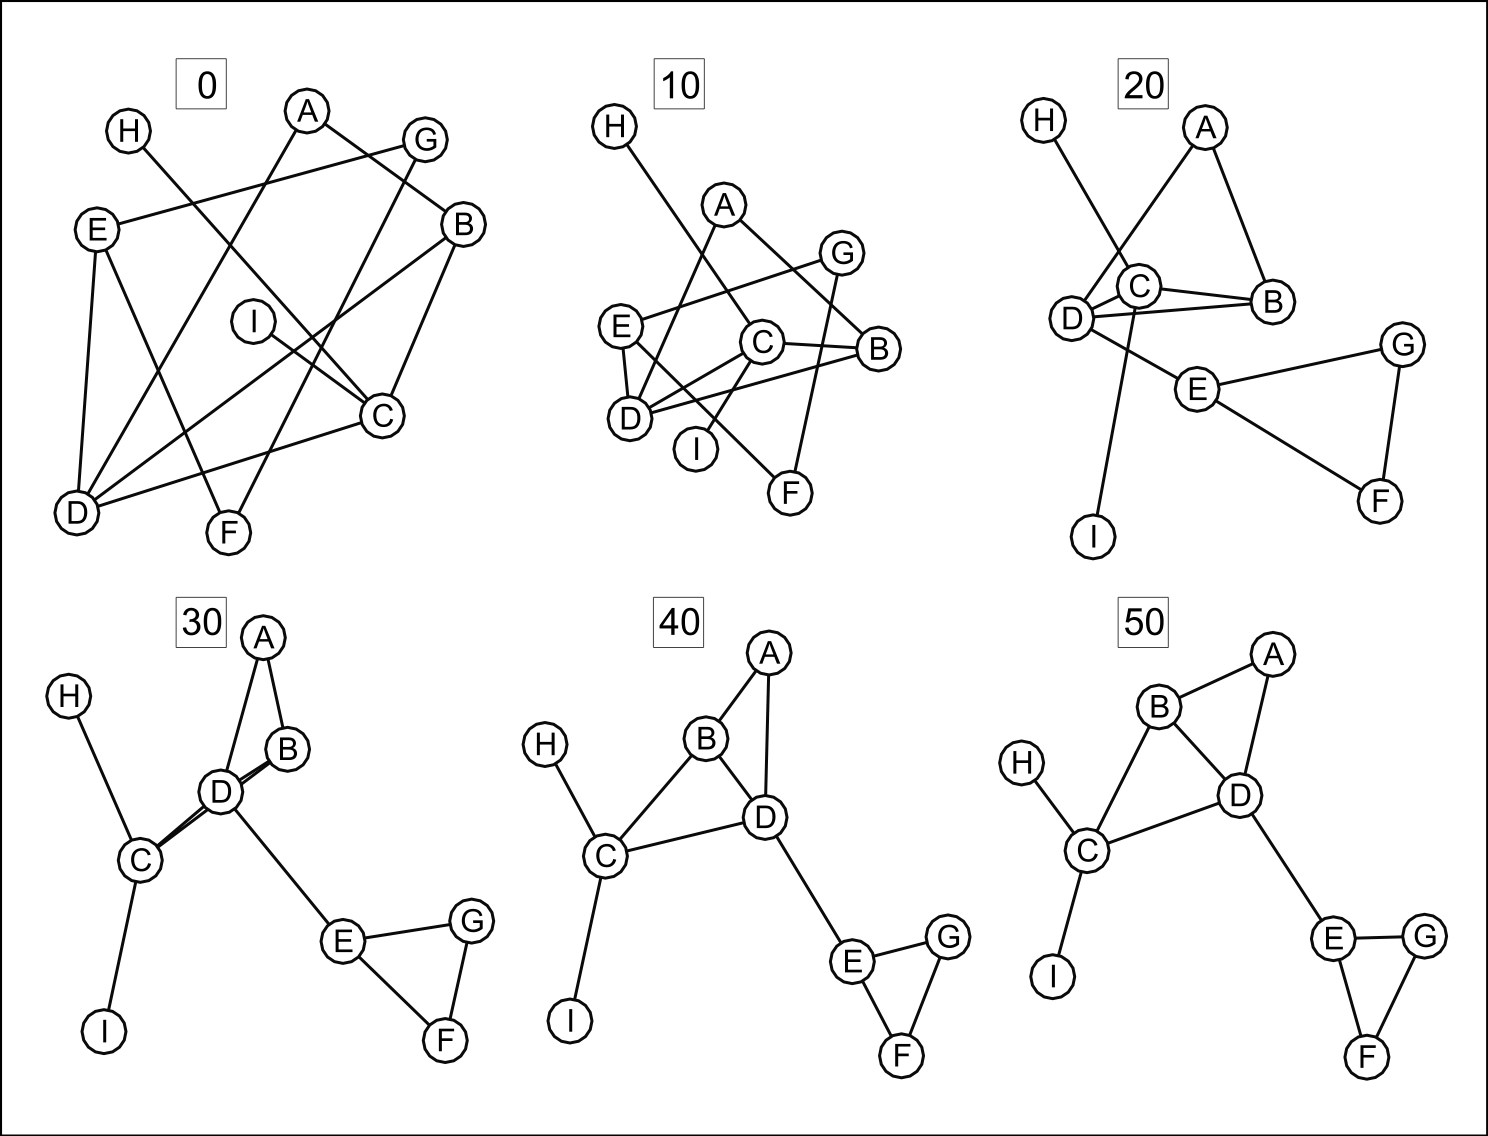
\includegraphics[width=\textwidth]{force-directed-layouts}
    \caption{Schrittweises Durchführen des Layout-Algorithmus von Fruchterman/Reingold}
    \bildquelle{Fruchterman, Thomas M. J./Reingold, Edward M.: Graph Drawing by Force-Directed Placement}
    \label{fig:force-directed-layouts}
\end{figure}

Force-Directed Layouts sind besonders effektiv für die übersichtliche
Darstellung von Netzwerken, in denen die Verbindungen zwischen den Elementen im
Vordergrund stehen. \parencite{schonfeld_fruchtermanreingold_2019} Im Gegensatz dazu
erfordert der Studiengangsfinder eine kontinuierliche Positionierung der
Studiengänge basierend auf inhaltlichen Ähnlichkeiten, was nicht unbedingt der
Stärke von Force-Directed Layouts entspricht. Force-Directed Graph Drawing
benötigt als Vorraussetzung bereits einen Graphen mit Knoten und Kanten, welche
im Fall des Studiengangsfinders die Ähnlichkeiten zwischen den einzelnen
Studiengängen entsprechen würde. Gerade die Berechnung der Ähnlichkeit zwischen
den einzelnen Studiengängen ist jedoch wesentlicher Bestandteil dieser Arbeit,
weshalb der Algorithmus nicht näher untersucht wurde.

\subsubsection{K-Means Clustering Algorithmus}
K-Means ist ein Clustering-Algorithmus, der Datenpunkte in $k$ vordefinierte
Gruppen oder Cluster einteilt. Die Wahl von $k$ stellt die Anzahl der Cluster dar,
und der Algorithmus versucht, die Datenpunkte so zu gruppieren, dass die Varianz
innerhalb der Cluster minimiert wird (siehe \autoref{fig:kmeans}).
\parencite{jeffares_k-means_2019}

\begin{figure}[H]
    \centering
    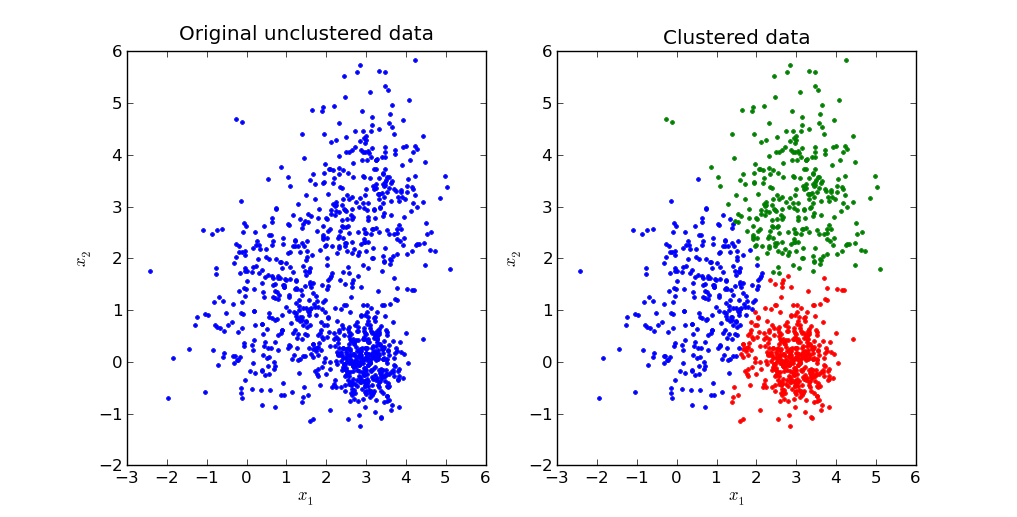
\includegraphics[width=\textwidth]{kmeans}
    \caption{K-Means Clustering Algorithmus}
    \bildquelle{https://mubaris.com/posts/kmeans-clustering/}
    \label{fig:kmeans}
\end{figure}

Die Entscheidung, den K-Means-Algorithmus nicht zu verwenden, basiert darauf, dass dieser hauptsächlich darauf abzielt, Datenpunkte zu gruppieren und weniger auf deren präzise Positionierung in einem zweidimensionalen Raum. Der Algorithmus fordert außerdem eine vordefinierte Clusteranzahl $k$. Das stellt im Falle des Studiengangsfinders jedoch keine Einschränkung dar, da jeder Cluster eine Inhaltskategorie, wie zum Beispiel \glqq Informatik\grqq{} repräsentieren würde. Dennoch ist der K-Means-Clustering-Algorithmus aufgrund seiner Empfindlichkeit gegenüber Ausreißern ungeeignet. Der Algorithmus versucht, Clusterzentren zu finden, die die Gesamtvarianz minimieren. Wenn es Ausreißer in den Studienschwerpunkten gibt, könnten sie das Ergebnis beeinflussen. \parencite{roth_demonstration_2023}

\subsubsection{Multidimensionale Skalierung (MDS)}\label{sec:MDS}
MDS ermöglicht die Reduktion $n$-dimensionaler Daten auf $m$-Dimensionen,
wodurch eine anschauliche Darstellung in Form von Koordinatenpaaren
ermöglicht wird \parencite{intro-to-multidimensional-scaling}. Dieser Aspekt ist
entscheidend, um Studiengänge in einem zweidimensionalen Diagramm zu
positionieren, wobei ähnliche Studiengänge aufgrund ihrer inhaltlichen
Ähnlichkeiten nahe beieinander liegen. Die Anwendung des MDS-Algorithmus auf
eine genormte Tabelle, in der im Falle von StudyMap die Studiengänge nach ihren
Anteilen an verschiedenen Inhaltskategorien gewichtet sind, ermöglicht eine
effektive Positionierung im Diagramm (siehe \autoref{table:input-mds}).

\begin{table}[!ht]
    \centering
    \begin{tabular}{|l|l|l|l|l|l|l|}
    \hline
        \textbf{Kürzel} & \textbf{Architektur} & \textbf{Gesundheit} & \textbf{Technik} & \textbf{Informatik} & \textbf{Wirtschaft} & \textbf{Internat.} \\ \hline
        \textbf{AT} & 0,55 & 0,06 & 0,09 & 0,04 & 0 & 0 \\ \hline
        \textbf{B} & 0,75 & 0 & 0 & 0,1 & 0 & 0,01 \\ \hline
        \textbf{ID} & 0,1 & 0,05 & 0,15 & 0,05 & 0,05 & 0 \\ \hline
        \textbf{HK} & 0,01 & 0,7 & 0,01 & 0,01 & 0,1 & 0,05 \\ \hline
        \textbf{PA} & 0 & 0 & 0,6 & 0,2 & 0,12 & 0,02 \\ \hline
        \textbf{IE} & 0 & 0 & 0,34 & 0,32 & 0,22 & 0,04 \\ \hline
        \textbf{LP} & 0 & 0,89 & 0,01 & 0 & 0,04 & 0,02 \\ \hline
        \textbf{SA} & 0 & 0,98 & 0 & 0 & 0 & 0 \\ \hline
        \textbf{IN} & 0 & 0 & 0,05 & 0,9 & 0 & 0,2 \\ \hline
        \textbf{IW} & 0 & 0 & 0,05 & 0,75 & 0,15 & 0,2 \\ \hline
        % \textbf{IM} & 0 & 0,2 & 0,1 & 0,65 & 0 & 0,05 \\ \hline
        % \textbf{BW} & 0 & 0 & 0 & 0 & 0,6 & 0,1 \\ \hline
        % \textbf{EB} & 0 & 0 & 0 & 0 & 0,5 & 0,4 \\ \hline
        % \textbf{SE} & 0 & 0 & 0,45 & 0,35 & 0,05 & 0,05 \\ \hline
        % \textbf{UI} & 0 & 0 & 0,36 & 0,12 & 0 & 0,04 \\ \hline
        % \textbf{MS} & 0 & 0 & 0,66 & 0,18 & 0 & 0,04 \\ \hline
        % \textbf{IR} & 0 & 0 & 0 & 0 & 0,1 & 0,8 \\ \hline
        % \textbf{REE} & 0 & 0 & 0,25 & 0,15 & 0,05 & 0,05 \\ \hline
        % \textbf{EI} & 0 & 0 & 0,5 & 0,25 & 0,05 & 0,05 \\ \hline
        % \textbf{ME} & 0 & 0 & 0,75 & 0,1 & 0,03 & 0,02 \\ \hline
        % \textbf{BE} & 0 & 0,07 & 0,6 & 0,12 & 0,11 & 0,06 \\ \hline
        % \textbf{MB} & 0 & 0 & 0,87 & 0,1 & 0,02 & 0 \\ \hline
        % \textbf{PT} & 0 & 0,95 & 0 & 0,03 & 0 & 0,09 \\ \hline
    \end{tabular}

    \caption{Exemplarische Eingabetabelle für den MDS-Algorithmus}
    \label{table:input-mds}
\end{table}

\autoref{table:input-mds} stellt eine stark vereinfachte Eingabetabelle für den
MDS-Algorithmus dar. Die erste Spalte enthält die Kürzel der verschiedenen
Studiengänge, wobei beispielsweise \textit{AT} für den Bachelor-Studiengang
Architektur steht. Die folgenden Spalten enthalten genormte Werte zwischen 0 und
1, die die prozentualen Anteile verschiedener Inhaltskategorien in den
jeweiligen Studiengängen repräsentieren. Diese genormten Werte werden im
n-dimensionalen Raum positioniert. Durch Anwendung des MDS-Algorithmus werden im
Verlauf die $n$-Dimensionen auf zwei Dimensionen reduziert, um schließlich eine
ästhetisch ansprechende Visualisierung in Form eines 2D-Diagramms zu generieren.

\noindent
Der klassische MDS-Algorithmus besteht aus den folgenden vier Schritten
\parencite{imperial_multidimensional_2019}:

% https://ceopedia.org/index.php/Multidimensional_scaling
\paragraph*{1. Berechnung der Distanzmatrix $ D_{ij} $}\label{sec:distanzmatrix}
Die Berechnung der Distanzmatrix $ D_{ij} $ erfolgt mithilfe des euklidischen
Abstands zwischen den Studiengängen im n-dimensionalen Raum. Der euklidische
Abstand zwischen zwei Punkten $ P_{i} $ und $ P_{j} $ wird nach der Formel

$$ d(P_i, P_j) = \sqrt{(x_i - x_j)^2 + (y_i - y_j)^2 + \ldots + (z_i - z_j)^2} $$

berechnet, wobei $ x_{i} $, $ y_{i} $, ..., $ z_{i} $ die Koordinaten von Punkt
$ P_{i} $ im $n$-dimensionalen Raum sind \parencite{ceopedia_multidimensional_2018}. Für die
Studiengangsdaten bedeutet das, dass die $n$-Dimensionen die verschiedenen
Inhaltskategorien repräsentieren.

Die euklidische Distanzmatrix $ D_{ij} $ enthält dann die euklidischen Abstände
zwischen jedem Paar von Studiengängen. In der Matrix sind die Elemente
$ D_{ij} $ die Distanzen zwischen den Studiengängen $ i $ und $ j $. Je näher
die Studiengänge in der Distanzmatrix beieinander liegen, desto näher werden sie
im finalen Diagramm platziert und umgekehrt.

Konkret in Python implementiert, sieht die Berechnung der Distanzmatrix wie
folgt aus:

\begin{lstlisting}[style=Python]
def calculate_distance_matrix(X):
    euclidean = lambda x,y:ma.sqrt(np.sum((np.array(x)-np.array(y))**2))
    D = []
    for x in X:
        tmp = []
        for y in X:
            tmp.append(euclidean(x, y))
        D.append(tmp)
    return D
\end{lstlisting}

% https://dorianhe.github.io/Intro-to-Multidimensional-Scaling/
% https://ceopedia.org/index.php/Multidimensional_scaling
% https://www.hongfeili.com/files/paper100/paper4.pdf
\paragraph*{2. Anwendung der Centering Matrix $ C $ zur Normalisierung der
Distanzen}
Die Formel $ C = I - \frac{1}{n} \vec{e} * \vec{e}^T $ berechnet die sogenannte Centering Matrix. $ I $ ist die Einheitsmatrix, $ \frac{1}{n} $ ist der Kehrwert der Anzahl der Datenpunkte und $ \vec{e} $ ist ein Vektor gefüllt mit Einsen. Das Symbol $ \vec{e}^T $ bezeichnet wie in der Mathematik üblich die Transposition des Vektors. \parencite{wickelmaier_introduction_2003}

Die Centering Matrix $ C $ wird verwendet, um die Distanzmatrix $ D $ zu
zentrieren. Das Zentrieren ist wichtig, um die Distanzen zwischen den Punkten
in der $n$-dimensionalen Raummatrix zu normieren und somit den Schwerpunkt der
Daten im Raum zu korrigieren. \parencite{wickelmaier_introduction_2003}

Schließlich wird diese eingesetzt um die Zentriermatrix $ B $ aus der
Distanzmatrix zu berechnen:
$$ B = - \frac{1}{2} * C * D_{ij} * C $$

\paragraph*{3. Spektralzerlegung}
Die Matrix $ B $ wird nun spektral zerlegt, um die Eigenwerte $ \lambda_{i} $
und die zugehörigen Eigenvektoren $ v_{i} $ zu erhalten.
$$ B = W * \Lambda * W^-1 $$
Hierbei ist $ W $ die Matrix der Eigenvektoren und $ \Lambda $ ist eine
Diagonalmatrix mit den Eigenwerten auf der Hauptdiagonale. Die Eigenvektoren
werden anschließend sortiert und die größten positiven Eigenwerte
$ \lambda_{1} ... \lambda{m} $ mit dazugehörigen Eigenvektoren
$ v_{1} ... v_{m} $ aus B extrahiert. \parencite{wickelmaier_introduction_2003}

\paragraph*{4. Projektion der Datenpunkte}
Um nun die Datenpunkte von einem höherdimensionalen Raum (basierend auf den
Beziehungen in der Distanzmatrix $ D $) auf einen niedrigdimensionalen Raum,
der durch die Eigenvektoren und Eigenwerte repräsentiert wird, abzubilden,
benötigt man folgende Projektion \parencite{he_classical_2018}:
$$ X = V_m \Lambda^{1/2}_m $$
Die Variable $ m $ steht für die Anzahl der gewünschten Dimensionen. Im Falle
von StudyMap entspricht $ m = 2 $, um das Ergebnis in einem 2D-Diagramm zu
visualisieren. $ V_{m} $ steht für die Eigenvektoren und $ \Lambda $ wie bereits
im vorherigen Absatz beschrieben für die Diagonalmatrix mit den Eigenwerten.
\parencite{wickelmaier_introduction_2003}

Abschließend enthält $ X $ die Matrix mit den auf $ m $-Dimensionen reduzierten
Koordinaten, welche dann z.B. in einem Diagramm visualisiert werden können.
An dieser Stelle wird für die Berechnung der Studiengänge (mit $ m = 2 $)
ermöglicht, dass innerhalb einer 2D-Darstellung, ähnliche Studiengänge aufgrund
ihrer inhaltlichen Ähnlichkeiten nahe beinander positioniert werden. Diese
räumliche Anordnung erleichtert die intuitive Analyse von Beziehungen zwischen
den einzelnen Bachelor- und Masterstudiengängen.

Insgesamt erfüllt der MDS-Algorithmus die spezifischen Anforderungen des
Studiengangsfinders, indem er eine übersichtliche und interpretierbare
Visualisierung der Studiengänge basierend auf inhaltlichen Ähnlichkeiten
ermöglicht.

\subsection{Beschreibung der Datenquelle und -beschaffung}
\subsubsection{Herkunft der Daten}\label{sec:herkunft-der-daten}
Die Grundlage für den Studiengangsfinder wurde in enger Zusammenarbeit mit Frau
Rösel, der Vizepräsidentin der Hochschule Regensburg, gelegt. Wir initiierten
den Prozess durch die Definition klarer Anforderungen an die benötigten
Informationen. Dazu gehört unter anderem die Definition der Inhaltskategorien
der Studiengänge. Der erste Entwurf entsprach folgender Aufteilung:

\begin{enumerate}
    \item Architektur und Bau
    \item Design und Medien
    \item Gesundheit und Soziales
    \item Technik
    \item Informatik und Mathematik
    \item Marketing und Kommunikation
    \item Erneuerbare Energien, Nachhaltigkeit und Umwelttechnik
    \item Wirtschaft und Management
    \item Internationales
\end{enumerate}

Diese Anforderungen wurden dann innerhalb der Hochschule kommuniziert und von
einer Teilmenge der Studiendekane für vereinzelte Studiengänge ausgefüllt. Das
heißt konkret, dass für 22 Studiengänge jeweils für alle dieser
Inhaltskategorien ein Wert festgelegt wurde.

Frau Rösel bleibt bis zur Übergabe der Arbeit weiterhin für die Beschaffung der Daten verantwortlich. Eine systematische Bewertung aller Studiengänge anhand des Modulplans und der jeweiligen ECTS pro Inhaltskategorie wird von Frau Rösel in Zusammenarbeit mit den Studiengangsverantwortlichen entwickelt.

Das European Credit Transfer System (ECTS) ist ein System zur Normierung von Studienleistungen innerhalb des Europäischen Hochschulraums. Dadurch können Unterschiede zwischen nationalen Hochschulsystemen ausgeglichen werden. \parencite{european_commission_europaisches_nodate} Jedes Fach an der OTH Regensburg hat eine bestimmte Anzahl von Credits (ECTS), die sich nach der Intensität des Faches richtet.

Die Bewertung des Studiengangsfinders erfolgt auf Basis der Inhaltskategorien und wird nun neutral nach der ECTS-Anzahl der jeweiligen Kategorie berechnet. So wird eine objektive Einstufung der Studiengänge für den verwendeten MDS-Algorithmus gewährleistet. Durch objektive Berechnungen ist es in Zukunft denkbar, die Aufgabe der Datenaktualisierung an eine dritte Person zu delegieren.

\subsubsection{Festlegung der Inhaltskategorien}
Im nächsten Schritt werden die Werte auf die Zeile normiert. Das heißt, die
Summe aller Inhaltskategorie-Werte pro Studiengang beträgt eins.

Im Umkehrschluss bedeutet das jedoch, dass die Studiengänge aufgrund von
Überschneidungen in den Kategorien nicht korrekt abgebildet werden können.
Beispiel:

\begin{table}[!ht]
    \centering
    \begin{tabular}{|l|l|l|l|l|}
    \hline
    \textbf{Studienfeld}           & \textbf{...} & \textbf{Informatik und Mathematik} & \textbf{Internationales} & \textbf{...} \\ \hline
    Informatik                     & ...          & 0,8                                & 0,2                      & ...          \\ \hline
    International Computer Science & ...          & 0,4                                & 0,6                      & ...          \\ \hline
    \end{tabular}

    \caption{Aufteilung der Werte bei auf Studiengang genormte Werte}
    \label{table:norm-values}
\end{table}

Tabelle \ref{table:norm-values} zeigt die Problematik der Überschneidungen. Der
Studiengang International Computer Science ist von den Inhalten nahezu
identisch zum Studiengang Informatik. Der Hauptunterschied ist, dass die Fächer
in Englisch angeboten werden. Dies hat zur Folge, dass der Studiengang
eigentlich sowohl in der Kategorie Informatik und Mathematik, als auch in der
Kategorie Internationales einen hohen Wert benötigt. Da die Zeilensumme eins
beträgt, ist dies nicht realistisch abbildbar. Aus diesem Grund wurde
entschieden die Werte pro Zelle, d.h. pro Kategorie und Studiengang auf eins
zu normieren. Mit dieser Aufteilung, kann ein Studiengang sowohl in Informatik
und Mathematik beispielsweise einen Wert von 0,8 haben, als auch in der
Kategorie Internationales.

Die anfängliche Kategorisierung der Studiengänge in neun allgemeine
Inhaltskategorien stellte sich als unzureichend heraus, da nach der Anwendung
des MDS-Algorithmus viele Studiengänge überlappend dargestellt wurden. Diese
Herausforderung führte zu einer entscheidenden Überarbeitung des
Kategorisierungssystems, um präzisere und differenzierte Bewertungen zu
ermöglichen. Die Lösung bestand in der Einführung von sogenannten Supergruppen,
die eine tiefere Bewertung der Studiengänge ermöglichten.

Ursprünglich waren Studiengänge wie \textit{Architektur} und
\textit{Bauingenieurwesen} in einer einzigen Kategorie
\textit{Architektur und Bau} zusammengefasst. Die Neuerung bestand darin, diese
in separate Kategorien wie \textit{Architektur} und \textit{Bau} zu unterteilen.
Ein zusätzliches Feld in der Eingabedatei legte fest, welche dieser Kategorien
später in der Benutzeroberfläche zu einer Supergruppe zusammengeführt werden
sollten. Dieser Ansatz ermöglichte eine präzisere Bewertung von Studiengängen,
insbesondere bei Studiengängen wie \textit{Architektur} und
\textit{Bauingenieurwesen}. Hier konnte der Studiengang \textit{Architektur} als
mehr \textit{Architektur} und weniger \textit{Bau} bewertet werden, während es
bei \textit{Bauingenieurwesen} genau umgekehrt war. Vor dieser Anpassung konnte
nur ein Wert für \textit{Architektur und Bau} festgelegt werden.

Um die Benutzeroberfläche übersichtlich zu halten, wurden Supergruppen
eingeführt. Diese ermöglichen eine aggregierte Darstellung mehrerer Kategorien,
ohne die Benutzeroberfläche unnötig zu komplex zu gestalten. Frau Rösel brachte
entscheidende Impulse in diesen Prozess ein. Durch ihre Rückmeldung wurden
darüber hinaus neue Kategorien wie \textit{Sprachkompetenzen},
\textit{Digitalität} und \textit{Future Skills} eingeführt. Diese dienen dazu,
eine noch präzisere Differenzierung und Bewertung der Studiengänge zu
ermöglichen. Folgende Liste zeigt die neuen Kategorien - jeder Listeneintrag
enthält dabei eine Supergruppe mit einem oder mehrere Kategorien:

\begin{enumerate}
    \item Architektur, Bau (Architektur und Bau)
    \item Design, Medien (Design und Medien)
    \item Gesundheit, Soziales (Gesundheit und Soziales)
    \item Maschinenbau, Elektrotechnik (Technik)
    \item Informatik (Informatik)
    \item Naturwissenschaften, Mathematik (Naturwissenschaften und Mathematik)
    \item Marketing, Kommunikation (Marketing und Kommunikation)
    \item Erneuerbare Energien, Umwelttechnik (Erneuerbare Energien und
    Umwelttechnik)
    \item Nachhaltikeit (Nachhaltigkeit)
    \item Wirtschaft, Management (Wirtschaft und Management)
    \item Sprachkompetenzen (Sprachkompetenzen)
    \item Digitalität (Digitalität)
    \item Future Skills (Future Skills)
\end{enumerate}

Die neuen Kategorien, ergänzt durch die Einführung der Supergruppen, schaffen
eine optimierte Grundlage für den MDS-Algorithmus. Dieser kann nun Studiengänge
präziser positionieren, da die Unterscheidungen und Bewertungen auf einer
feineren Ebene vorgenommen werden. Diese Anpassungen tragen entscheidend dazu
bei, das Ziel einer verfeinerten Studienorientierung und -wahl zu erreichen.
\newpage

% Konzept und Umsetzung an der OTH-Regensburg
\section{Konzept und Umsetzung an der OTH-Regensburg}

\subsection{Vorstellung der OTH-Regensburg als Fallbeispiel}

\subsection{Konzept für eine automatisch generierte Infografik}

\subsection{User-centered Design Research: Mockup eines Prototypen}

\subsection{Beschreibung der Positionsberechnung der Infografik}

\subsection{Technische Details zur Umsetzung}

\subsection{Anwendung des entwickelten Systems auf die Studiengänge der OTH-Regensburg}
\newpage

% Mockup-, und Prototypen-Studie
\section{User-centered Design Research}

\subsection{Mockup-Studie: Bewertung der Benutzerfreundlichkeit und
Funktionalität}
Bei der Entwicklung eines nutzerzentrierten Designs steht die direkte Einbindung
der Zielgruppe im Mittelpunkt. Dieser Ansatz, der als User-Centered Design (UCD) 
bezeichnet wird, stellt die Integration der Bedürfnisse, Erwartungen und
Anforderungen der Benutzer in den Entwicklungsprozess in den Mittelpunkt. Ziel
ist es, Produkte und Anwendungen zu gestalten, die nicht nur funktional und
ästhetisch ansprechend sind, sondern auch die bestmögliche
Benutzerfreundlichkeit bieten.

\subsubsection{Methodik und Teilnehmende}
Im Rahmen des UCD-Prozesses wurde das zuvor in Kapitel \ref{sec:konzept}
vorgestellte Mockup-Konzept für den Studiengangsfinder entwickelt, das als
Prototyp diente. Um sicherzustellen, dass das entworfene Konzept den
Bedürfnissen der potenziellen Nutzer entspricht, wurde eine gezielte 
User-Centered-Design-Studie durchgeführt. Zu diesem Zweck wurden sechs
Studierende und Absolventen verschiedener Fachrichtungen eingeladen, den
Mockup-Entwurf zu evaluieren (siehe \autoref{table:teilnehmer-mockup-studie}).

\begin{table}[!ht]
    \centering
    \begin{tabular}{|l|l|l|l|}
        \hline
        \textbf{\#} & \textbf{Studienabschluss}                               & \textbf{Geschlecht} & \textbf{Datum} \\ \hline
        1           & Betriebswirtschaft B.A.                                 & Weiblich            & 16.09.2023     \\ \hline
        2           & Psychologie M.Sc.                                       & Weiblich            & 20.09.2023     \\ \hline
        3           & Informatik B.Sc.                                        & Männlich            & 25.09.2023     \\ \hline
        4           & Regenerative Energietechnik und Energieeffizienz B.Eng. & Männlich            & 07.10.2023     \\ \hline
        5           & Bioprozessinformatik B.Sc.                              & Männlich            & 08.10.2023     \\ \hline
        6           & Betriebswirtschaft B.A.                                 & Weiblich            & 12.10.2023     \\ \hline
    \end{tabular}

    \caption{Probanden der Mockup-Studie}
    \label{table:teilnehmer-mockup-studie}
\end{table}

\subsubsection{Ablauf des Tests}
Die Studie wurde in Form von Einzelinterviews durchgeführt. Die Teilnehmer wurden ermutigt, ihre persönlichen Perspektiven, Erfahrungen und Vorschläge einzubringen. Außerdem wurden sie gebeten, ihre Gedanken zum Entwurf laut zu äußern. Anschließend wurden ihnen nacheinander alle Grafiken des Entwurfs gezeigt (1. \autoref{fig:mockup-bubbles},
2. \autoref{fig:mockup-bubbles-hover}, 3. \autoref{fig:mockup-bubbles-popup}). 

Offene Fragen zu Designelementen, Verständlichkeit von Informationen und allgemeinen Nutzererfahrungen sollten Aufschluss über mögliche Stärken und Schwächen des Design-Proto\-typs geben. Ziel war es, frühzeitig wertvolles Feedback zu erhalten, um Optimierungen und Anpassungen vornehmen zu können, bevor die Umsetzung in die nächste Phase geht. Die lauten Gedanken der Teilnehmerinnen und Teilnehmer wurden von Herrn Huber in einem Freitextfeld dokumentiert.

\subsubsection{Ergebnisse der Mockup-Studie}
Die Rückmeldungen der Studienteilnehmenden lassen sich in folgende konsistente
Muster zusammenfassen.

\paragraph{Bild 1: Visualisierung der Studiengänge}\label{sec:visualisierung-der-studiengänge}
Die Übersichtskarte wurde von den Teilnehmenden als unübersichtlich und geclustert wahrgenommen. Besonders die Farbähnlichkeit der Studiengänge wurde als störend
empfunden.

Eine konkrete Verbesserungsmöglichkeit besteht darin, die Überschriften der Nebel zu vergrößern und fett darzustellen, um die Lesbarkeit zu verbessern. Darüber hinaus wurde vorgeschlagen, alle Abkürzungen der Studiengänge standardmäßig auszublenden und nur den Nebel zu beschriften, um die Übersichtlichkeit zu erhöhen. Sobald der Benutzer mit der Maus in die Nähe des Nebels kommt, sollte die Überschrift des Nebels ausgeblendet und die Abkürzungen aller darin enthaltenen Studiengänge eingeblendet werden. Um die Zufälligkeit und Ähnlichkeit der Farben zu vermeiden, könnten die Studiengänge in den Fakultätsfarben und der Nebel im Hintergrund neutral (z.B. grau) eingefärbt werden.

\paragraph{Bild 2: Interaktivität}
Das Hover-Event über eine Bubble mit einem Tooltip wurde durchweg als passend und verständlich betrachtet. Dieses Element wurde von den Teilnehmenden als intuitiv und funktional empfunden.

\paragraph{Bild 3: Popup mit Details eines Studiengangs}
Über die Anordnung der Informationen im Popup gingen die Meinungen auseinander. Während einige eine absteigende Sortierung nach Relevanz bevorzugten, sprachen sich andere für eine alphabetische Sortierung aus. Positiv bewertet wurde die Funktion, ähnliche Studiengänge nach Ähnlichkeit zu sortieren. Die Darstellung der Branchen wurde als weniger aussagekräftig empfunden und teilweise vorgeschlagen, diese Information zu entfernen. Die Möglichkeit, sich Unternehmen in Regensburg anzeigen zu lassen, wurde positiv bewertet und es wurde angeregt, diese Funktion ausklappbar zu gestalten, um die Übersichtlichkeit zu erhöhen. Es wurde außerdem empfohlen, die Informationen zu den Einstiegsgehältern zu erläutern, möglicherweise durch die Integration von Fragezeichensymbolen und Tooltips.

\paragraph{Generelle Anmerkungen}
Zu den allgemeinen Verbesserungsvorschlägen gehören ein besserer Farbkontrast, mehr Erläuterungen zu verschiedenen Informationen und eine einheitliche und intuitive Anordnung der Designelemente, um die Übersichtlichkeit insgesamt zu erhöhen.

%
%
%
%
%
%
% PROTOTYPEN STUDIE
\subsection{Prototypen-Studie: Evaluation durch Studieninteressierte}
Nach der Entwicklung des Prototyps auf Basis des Mockups und der Erkenntnisse aus der Mockup-Studie wurden Studieninteressierte eingeladen, den Prototyp von StudyMap zu testen. Nach der selbstständigen Interaktion mit dem Prototyp wurden die Teilnehmenden gebeten, an einer Umfrage teilzunehmen, um ihre Erfahrungen, Meinungen und Verbesserungsvorschläge zu dokumentieren.

Der folgende Abschnitt beleuchtet die Methodik, den genauen Ablauf des Tests und stellt die Ergebnisse dieser Evaluationsstudie vor, die wertvolle Einblicke in die Effektivität und Benutzerfreundlichkeit des Prototyps liefert.

\subsubsection{Methodik und Teilnehmende}
Der nächste Schritt im UCD-Prozess ist das Testen des Prototyps mit potenziellen Nutzern, d.h. Studieninteressierten. Zu diesem Zweck wurde auf der Grundlage des Mockups und der im vorherigen Kapitel beschriebenen Mockup-Studie ein Prototyp entwickelt (siehe \autoref{fig:prototyp-overview}). Ziel dieser Studie ist es, frühe Designentscheidungen zu hinterfragen und das Tool auf Usability zu testen. Der Vorteil einer solch frühen Evaluierung ist, dass größere Änderungen am Endprodukt wesentlich aufwendiger sind als in einem frühen Entwicklungsstadium.

\begin{figure}[H]
    \centering
    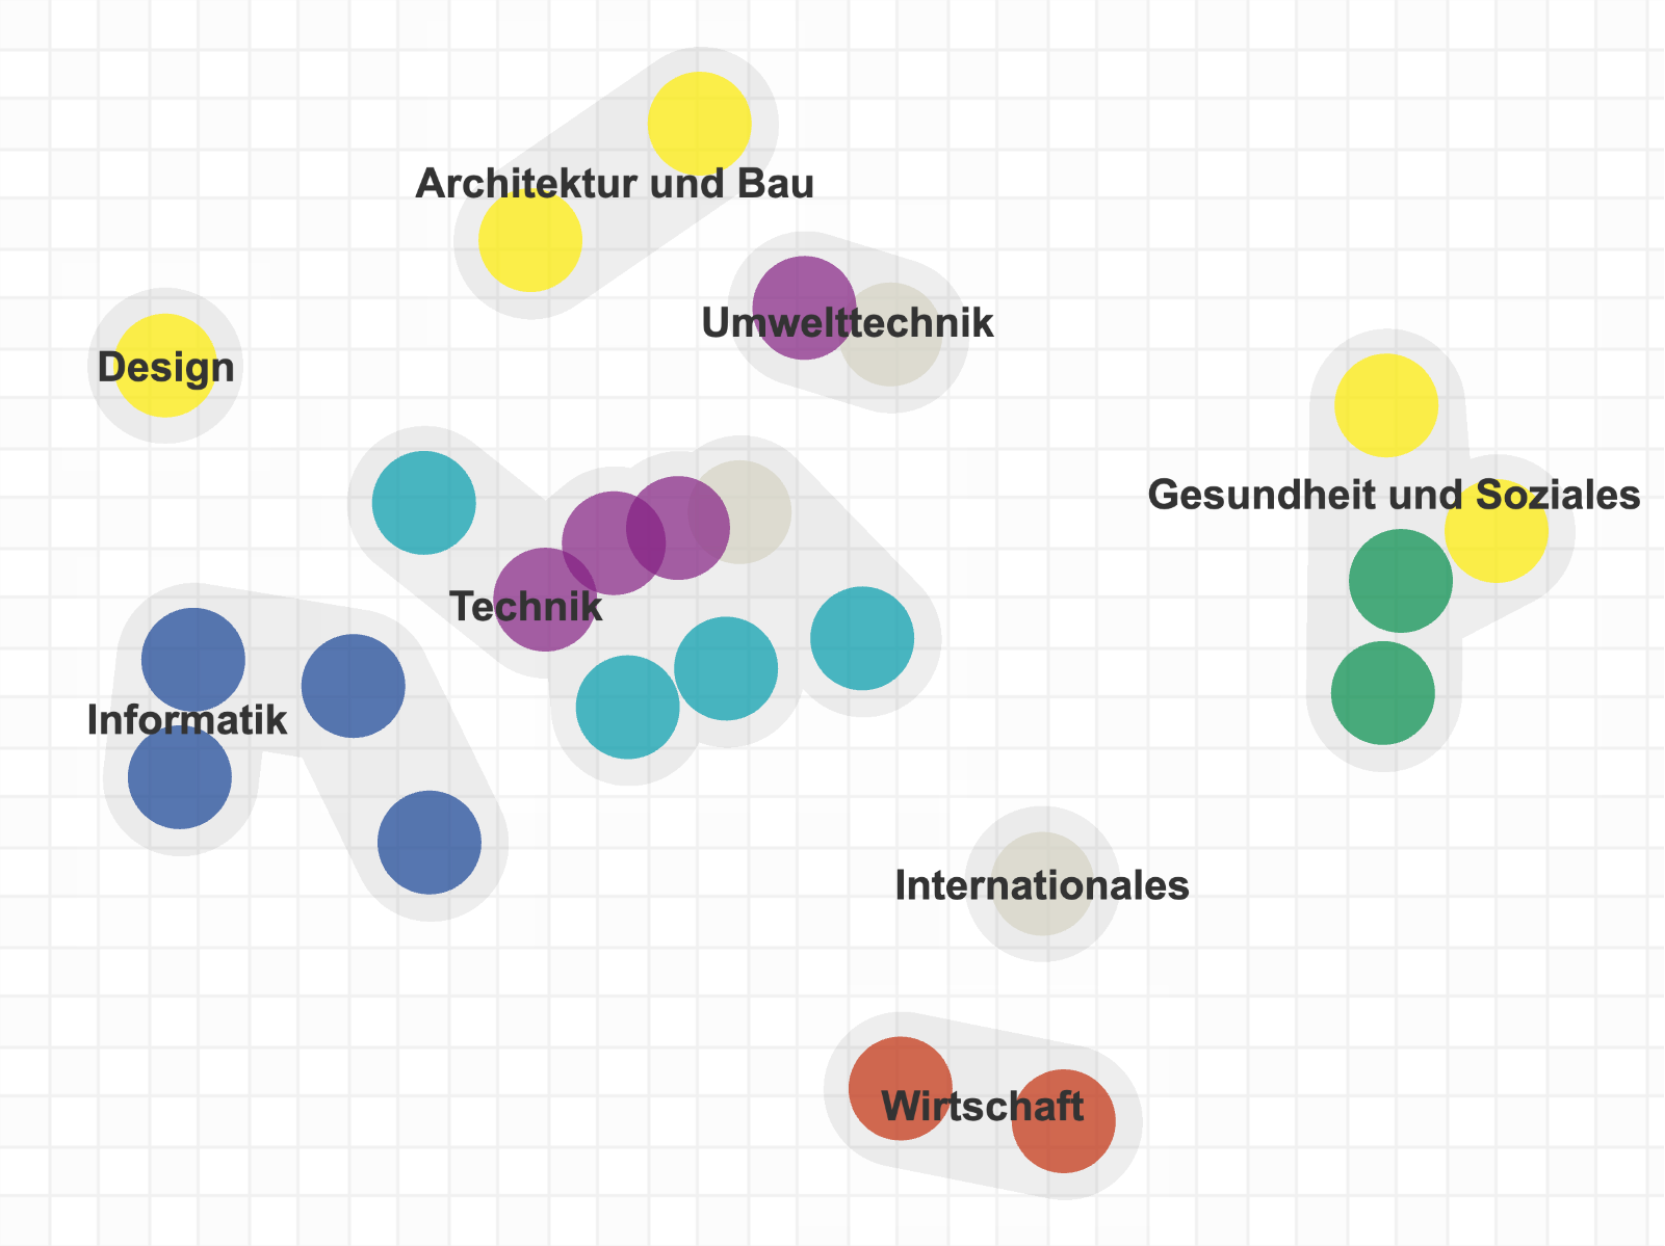
\includegraphics[width=\textwidth]{prototyp_overview}
    \caption{StudyMap Prototyp}
    \bildquelle{Eigene Darstellung}
    \label{fig:prototyp-overview}
\end{figure}

An der Studie nahmen 40 Schülerinnen und Schüler der 11. Klasse des Johannes-Nepomuk-Gymnasiums in Rohr i.NB teil. Alle diese Schüler werden voraussichtlich im Jahr 2026 die allgemeine Hochschulreife erlangen und entsprechen damit genau der Zielgruppe eines Studiengangfinders. Durch die örtliche Nähe des Gymnasiums zur OTH-Regensburg ist die Eignung des Teilnehmerkreises zusätzlich gegeben.

Die Befragung fand in zwei Gruppen (Klasse 11A und Klasse 11B) im Johannes-Neopomuk-Gymnasium vor Ort im Computerraum der Schule statt. Dort konnten die Schülerinnen und Schüler an den Windows-Rechnern der Schule sowohl den Prototyp testen als auch die Umfrage in Einzelarbeit beantworten.

\subsubsection{Ablauf des Tests}
Die Studie begann mit einer kurzen Einführung, in der den Teilnehmenden der
Zweck der Studie und die Handhabung des Prototyps erläutert wurden. Anschließend
wurden die Teilnehmenden gebeten, den Prototyp selbst zu verwenden und zwei
Aufgaben innerhalb einer Online-Umfrage zu lösen, um die Benutzerfreundlichkeit, die Navigationsstruktur und
die Funktionalitäten des Studiengangsfinders zu testen (siehe
\autoref{fig:prototyp-umfrage-aufgaben} - \textbf{Umfrage Teil 2}). In dieser Phase wurden sowohl
quantitative als auch qualitative Daten erhoben, um ein umfassendes Bild der 
Benutzererfahrung zu erhalten.

\begin{figure}[H]
    \centering
    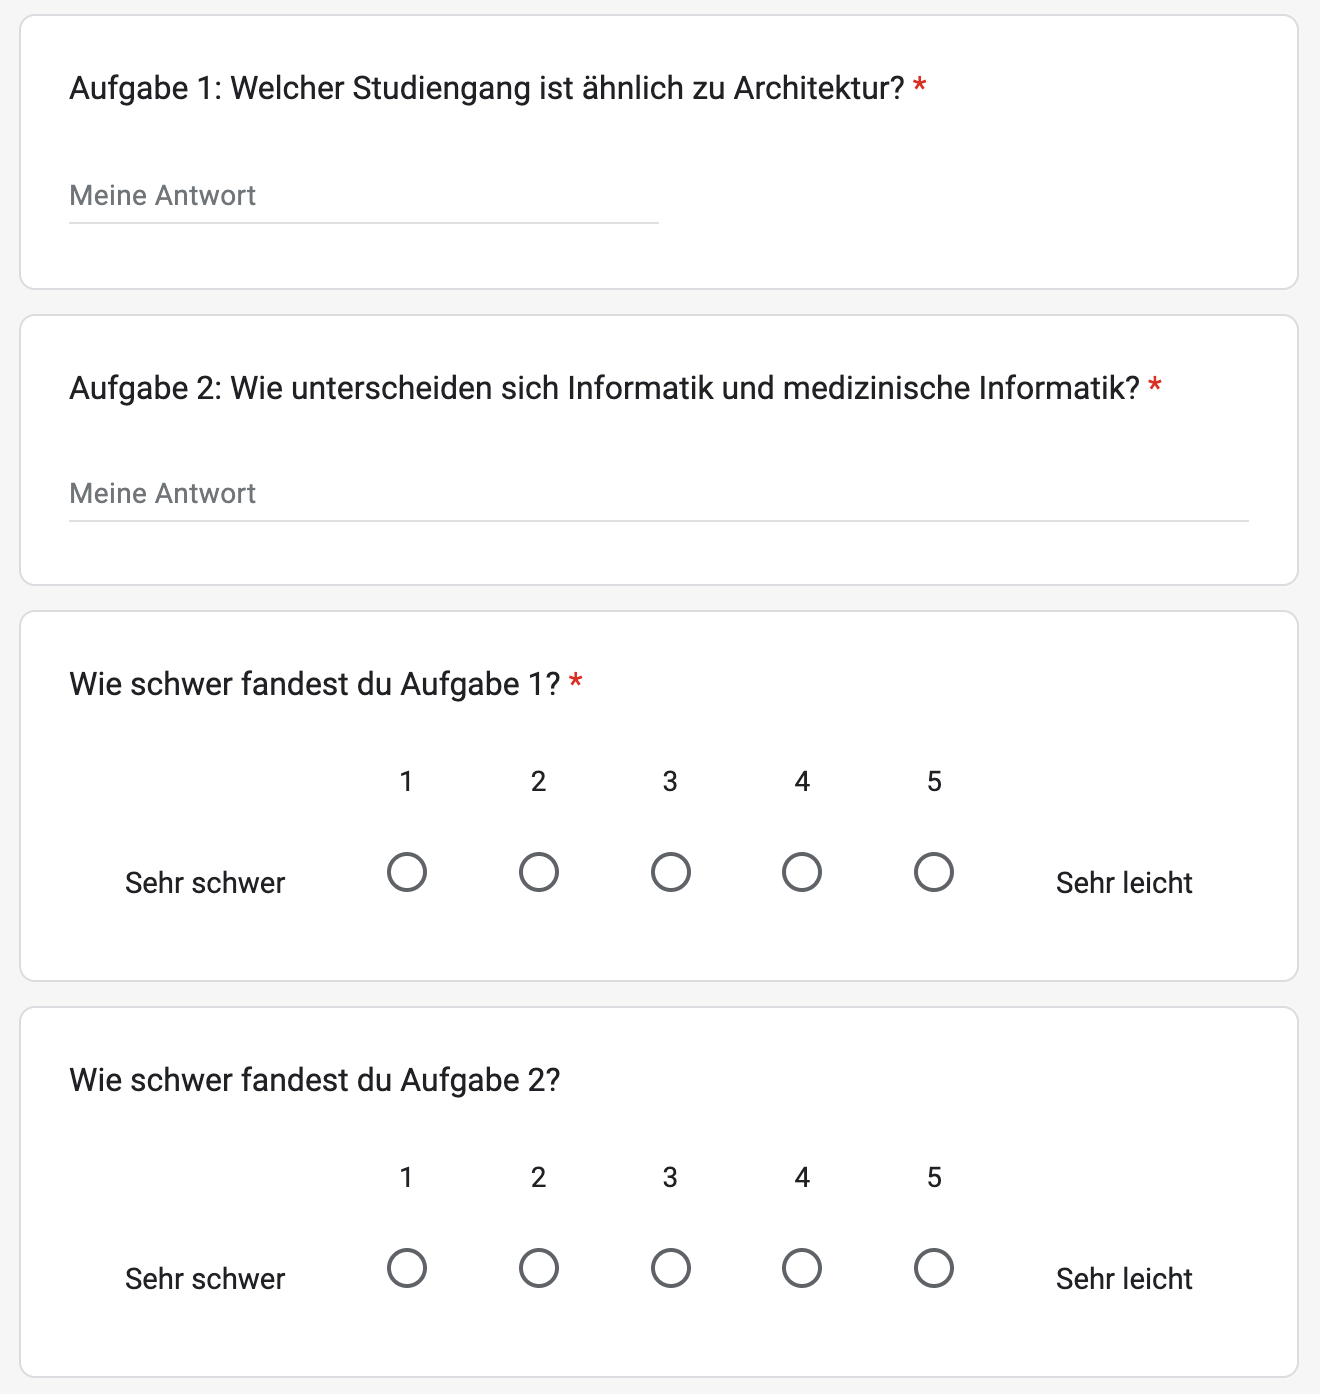
\includegraphics[width=0.5\textwidth]{umfrage_aufgaben}
    \caption{Prototypen-Studie: Aufgaben (Umfrage Teil 2)}
    \bildquelle{Eigene Darstellung}
    \label{fig:prototyp-umfrage-aufgaben}
\end{figure}

Nach der Interaktion mit dem Prototyp wurden die Teilnehmenden gebeten, zusätzlich zu den Aufgaben weitere Fragen in der anonymen Online-Umfrage zu beantworten.

Die ersten Fragen der Umfrage waren Multiple-Choice-Fragen mit den Antwortmöglichkeiten \glqq Ja\grqq{}, \glqq Nein\grqq{} und \glqq Keine Angabe\grqq{} \textbf{(Umfrage Teil 1)}.

\begin{enumerate}
    \item Willst du nach dem Abi studieren?
    \item Wenn ja, weißt du schon, was für ein Studium?
    \item Würde dir StudyMap bei der Wahl des Studiengangs helfen?
    \item Die Antwort hier ist \glqq Ja\grqq{} (Aufmerksamkeitsfrage)
\end{enumerate}

Danach folgten die beiden oben beschriebenen Aufgaben (siehe
\autoref{fig:prototyp-umfrage-aufgaben}). Zuletzt wurden die folgenden Fragen
mit Freitextfeldern zur Beantwortung gestellt \textbf{(Umfrage Teil 3)}:

\begin{enumerate}
    \item Was findest du an dem Konzept gut?
    \item Was findest du am Konzept schlecht?
    \item Hast du neue Ideen für den Prototyp?
    \item Wenn du bei \glqq Würde StudyMap dir bei der Studienwahl helfen?\grqq{} NEIN angekreuzt hast: Warum nicht?
\end{enumerate}

Die Fragen wurden bewusst mit Freitextfeldern zur Beantwortung versehen, um den Teilnehmenden die Möglichkeit zu geben, mit allen möglichen Gedankengängen zu antworten. Dies kann dazu führen, dass Ideen entstehen, die bisher noch nicht bedacht wurden und somit im Endprodukt umgesetzt werden können. Die Befragung dauerte ca. 15 Minuten. Durch die Kombination der Interaktion mit dem Prototyp und der schriftlichen Befragung konnten vielfältige Einblicke in die Nutzerperspektive gewonnen werden.

\subsubsection{Ergebnisse der Prototypen-Studie}

\paragraph{Umfrage Teil 1: Fragen}

\begin{figure}[H]
    \centering
    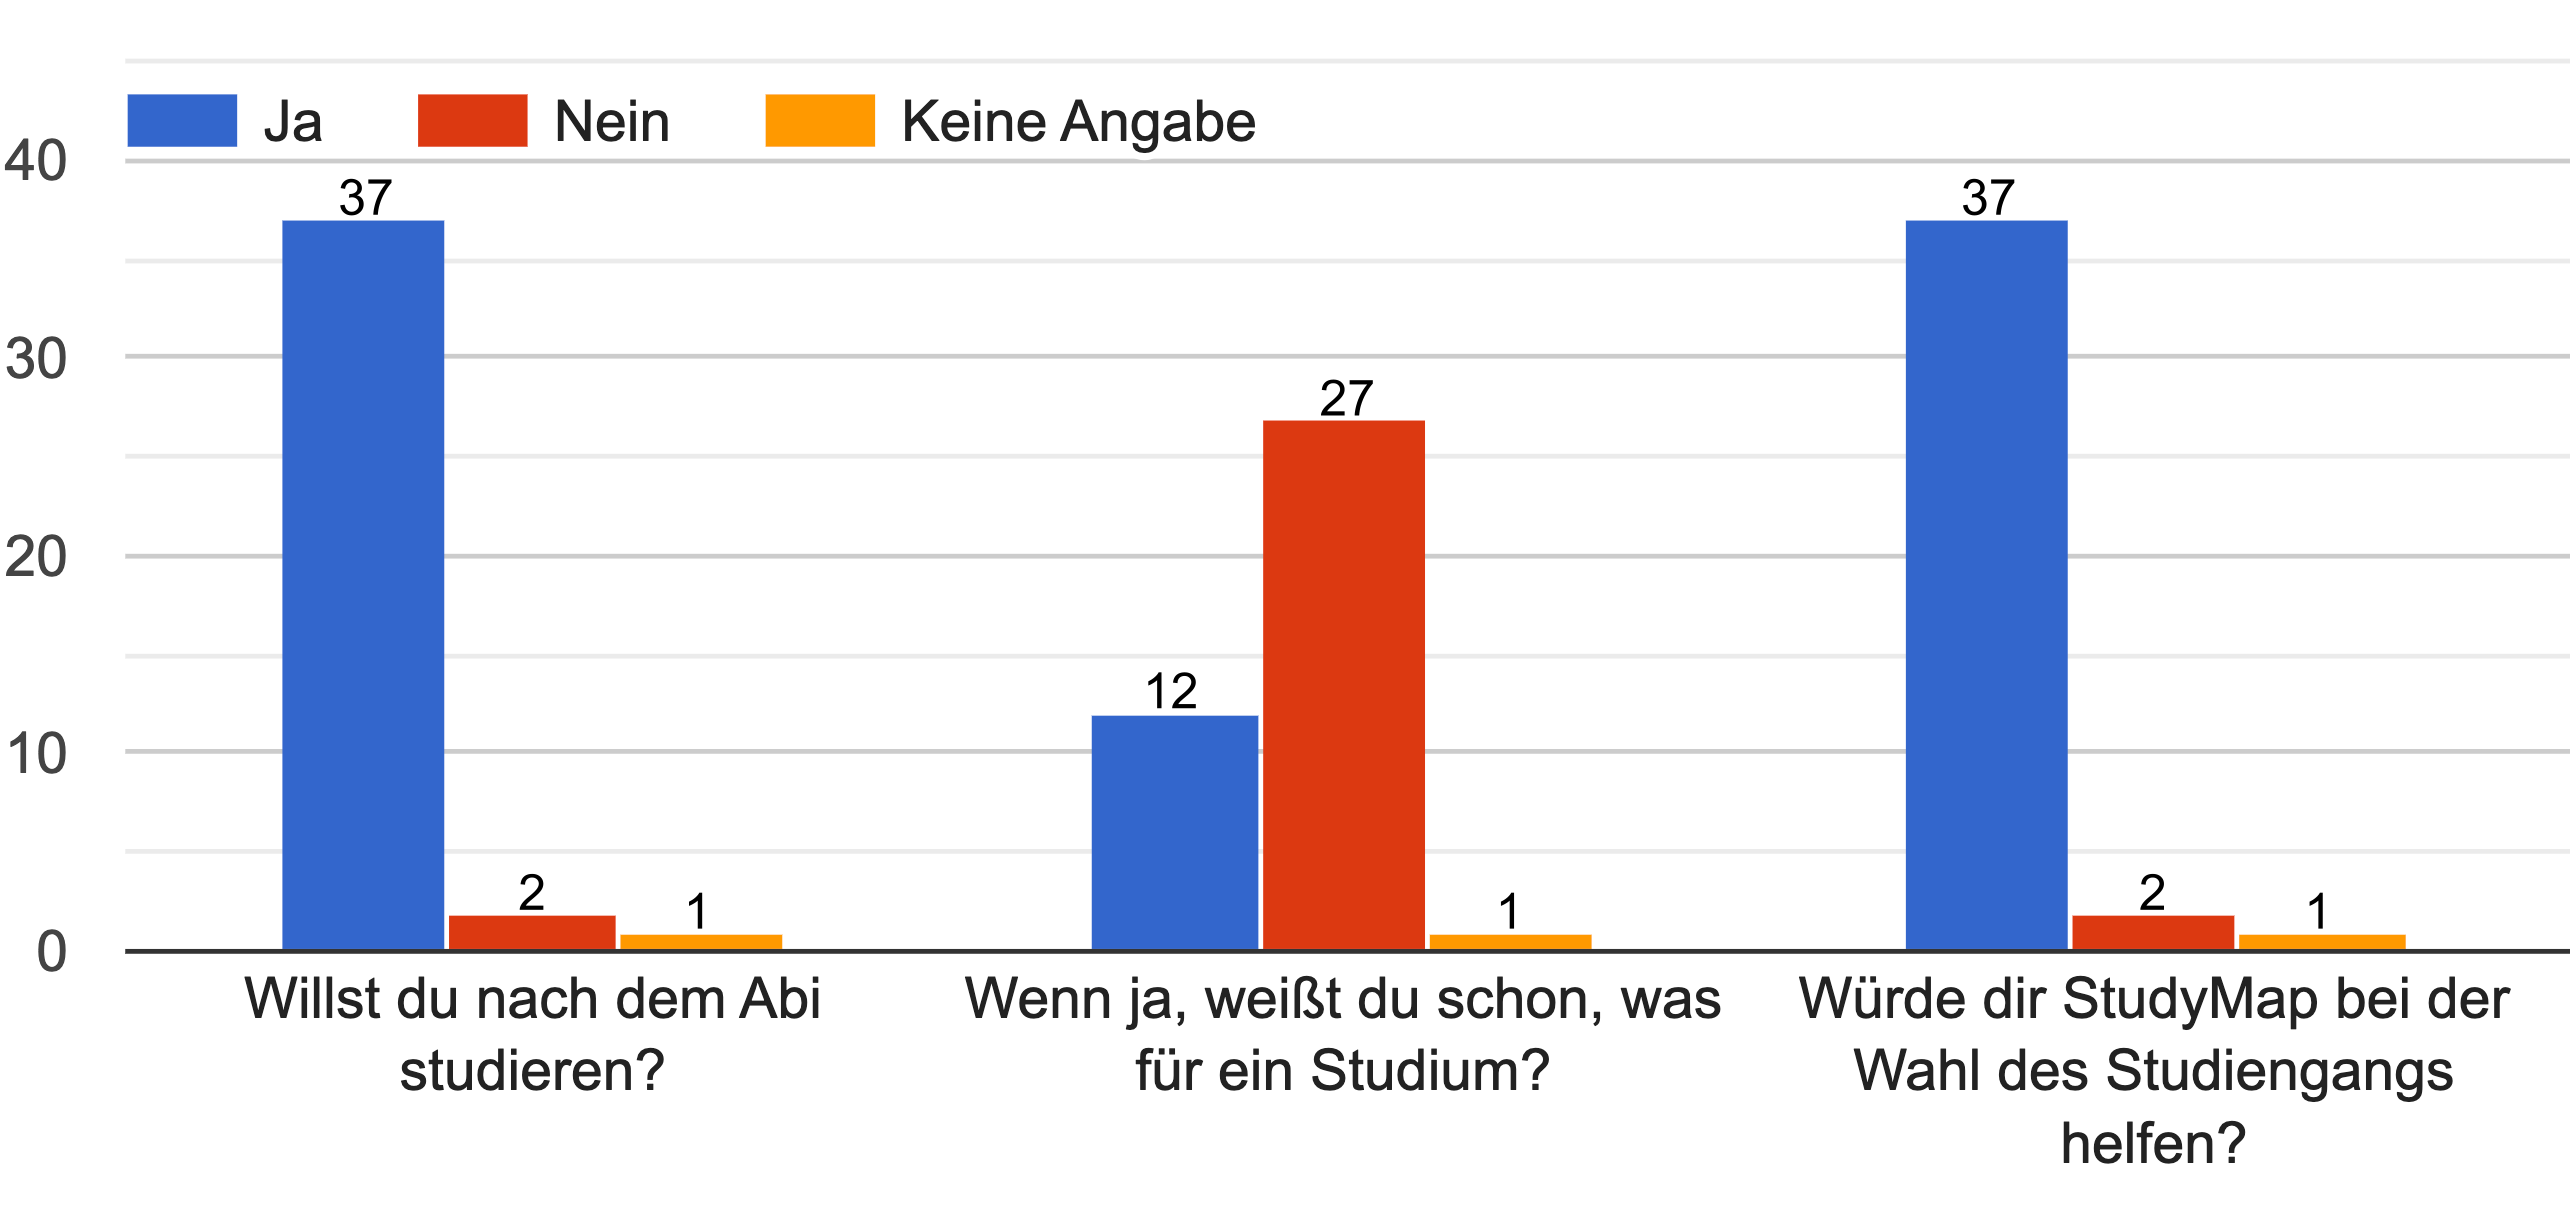
\includegraphics[width=\textwidth]{linien_fragen_1}
    \caption{Ergebnisse: Teil 1}
    \bildquelle{Google Forms + selbst ergänzte absolute Werte}
    \label{fig:linien-fragen-1}
\end{figure}

\autoref{fig:linien-fragen-1} zeigt, dass die erste Frage (\glqq Möchtest du nach dem Abitur studieren?\grqq{}) von 92,5 \% der Befragten bejaht wurde. Während zwei Personen (5 \%) die Frage verneinten, machte nur eine Person (2,5 \%) keine Angabe. Daraus lässt sich schließen, dass es sich bei der gewählten Teilnehmergruppe tatsächlich um die richtige Zielgruppe von StudyMap handelt.

Auf die Frage \glqq Wenn ja, weißt du schon, was du studieren willst?\grqq{} antworteten 30 \% (12) der Befragten mit \glqq Ja\grqq{}. 67,5 \% (27) haben mit \glqq Nein\grqq{} geantwortet und 2,5 \% haben wiederum die Angabe verweigert. Die Person, die bei Frage 1 angegeben hat, nicht zu antworten, hat bei dieser Frage mit \glqq Nein\grqq{} geantwortet. Die Person, die bei Frage 2 mit \glqq Keine Angabe\grqq{} stimmte, hatte zuvor bei Frage 1 mit \glqq Ja\grqq{} gestimmt. Die beiden Schüler, die bei Frage 1 mit \glqq Nein\grqq{} für ein Studium geantwortet haben, haben auch Frage 2 mit \glqq Nein\grqq{} votiert.

Zieht man die beiden Schülerinnen und Schüler, die sich bei Frage 1 gegen ein Studium entschieden haben, von den \glqq Nein\grqq{}-Antworten bei Frage 2 ab, so verbleiben 25 von 37 Studieninteressierten, die noch nicht wissen, was sie studieren werden. Daraus ergibt sich ein Anteil von 67,57 \% der Schüler der 11. Klasse, welche voraussichtlich nach dem Abitur eine Studienorientierung benötigen. Dieser Anteil an Schülern könnte mithilfe des innovativen Studiengangsfinders zu einem passenden Studiengang geführt werden.

Die dritte Frage (\glqq Würde dir StudyMap bei der Studienwahl helfen?\grqq{}) wurde von 37 von 40 Teilnehmern (92,5 \%) bejaht. Zwei Teilnehmer antworteten mit \glqq Nein\grqq{} und eine Person enthielt sich der Stimme. Im Falle einer Verneinung hatten die Befragten die Möglichkeit, dies im Anschluss in einem Freitextfeld zu begründen. Die beiden Personen, die mit \glqq Nein\grqq{} geantwortet haben, gaben an, dass StudyMap ihnen nicht bei der Studienwahl helfen würde, da sie bereits wüssten, was sie studieren wollen. Die Antworten auf diese Frage verdeutlichen noch einmal den Bedarf des Studiengangsfinders als Orientierungshilfe für Studieninteressierte.

Die Frage Nr. 4 der Umfrage Teil 1 wurde von allen Teilnehmern korrekt mit \glqq Ja\grqq{} beantwortet. Sie diente dazu, willkürlich ausgefüllte und damit nicht auswertbare Teilnahmen aus der Befragung auszusortieren.

\paragraph{Umfrage Teil 2: Aufgaben}

\begin{figure}[H]
    \centering
    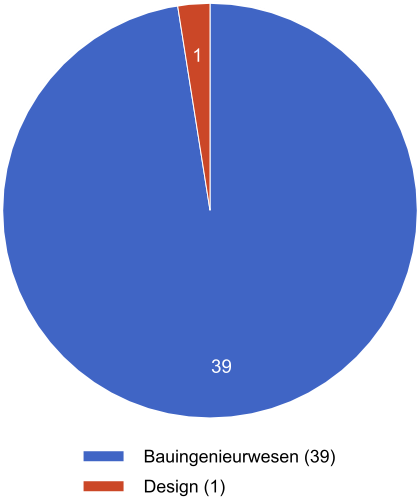
\includegraphics[width=0.4\textwidth]{torte_bauingenieur}
    \caption{Welcher Studiengang ist ähnlich zu Architektur? (Aufgabe 1)}
    \bildquelle{Eigene Darstellung}
    \label{fig:prototyp-umfrage-bauingenieur}
\end{figure}

In Aufgabe 1 sollten die Studienteilnehmer herausfinden, welcher Studiengang dem Studiengang "Architektur" ähnlich ist. Als Hilfsmittel stand ihnen der Live-Prototyp zur Verfügung. Wie in den vorherigen Kapiteln erläutert, werden ähnliche Studiengänge durch den MDS-Algorithmus nahe beieinander platziert. Die Lösung war daher der Studiengang \glqq Bauingenieurwesen\grqq{} (siehe \autoref{fig:prototyp-umfrage-bauingenieur-erklaerung}). 39 von 40 Studierenden (97,5 \%) lösten diese Aufgabe richtig. Die einzige falsche abgegebene Antwort entsprach dem Studiengang \glqq Design\grqq{}. \glqq Design\grqq{} ist im Prototyp eine Inhaltskategorie und kein Studiengang, ist aber tatsächlich dem Studiengang \glqq Architektur\grqq{} benachbart. Die hohe Übereinstimmung mit der Lösung weist auf die Intuitivität des Konzepts hin und stärkt damit die Basis für die weitere Entwicklung.

\begin{figure}[H]
    \centering
    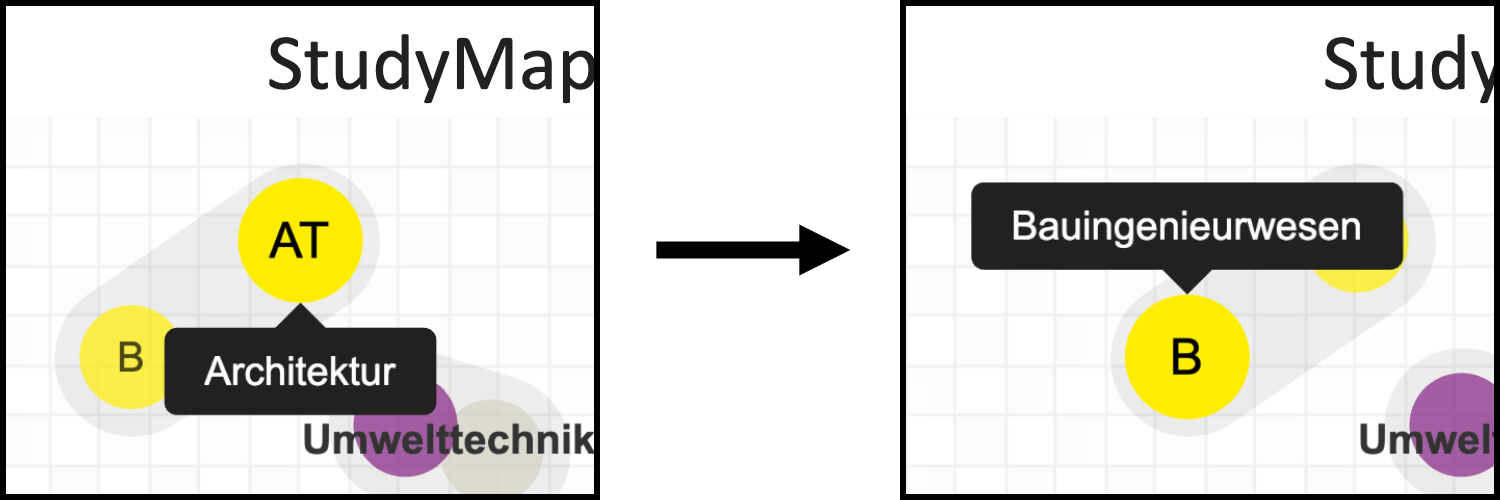
\includegraphics[width=0.65\textwidth]{prototyp_at_b}
    \caption{Prototyp: Architektur -> Bauingenieurwesen (Aufgabe 1)}
    \bildquelle{Eigene Darstellung}
    \label{fig:prototyp-umfrage-bauingenieur-erklaerung}
\end{figure}

%% Aufgabe 2

\begin{figure}[H]
    \centering
    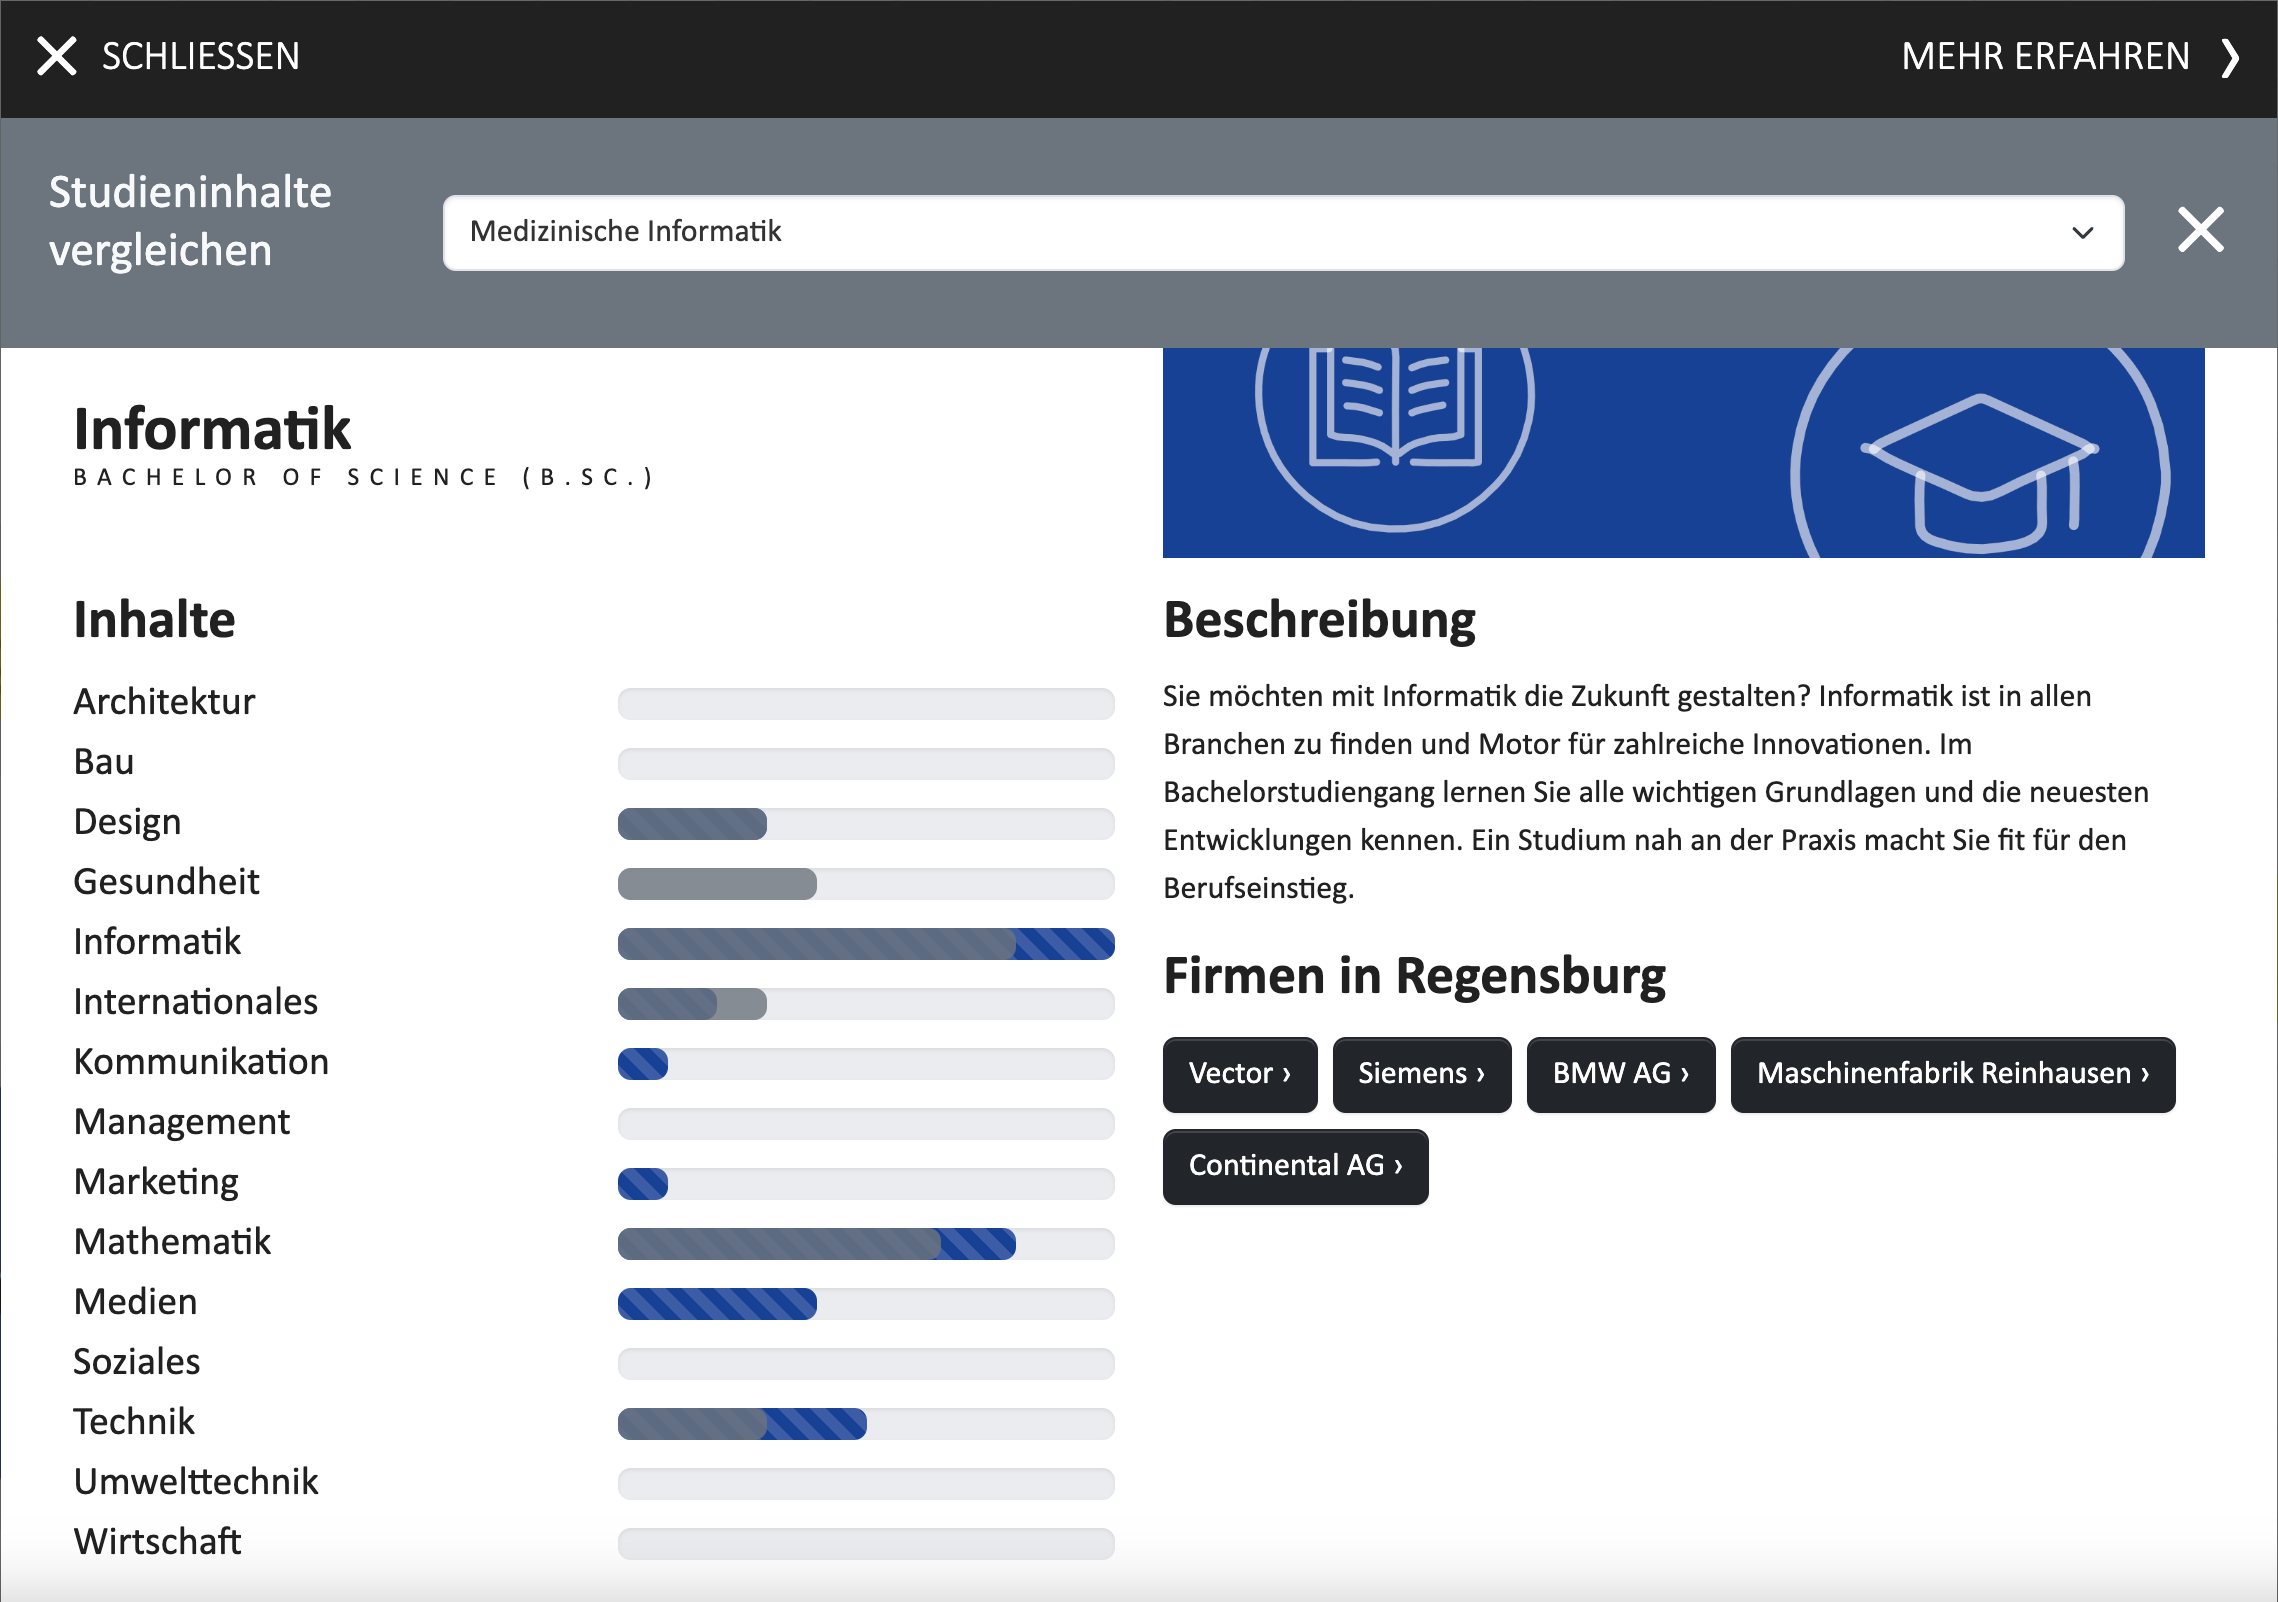
\includegraphics[width=\textwidth]{prototyp_comparison_i_im}
    \caption{Prototyp: Vergleichsfeature}
    \bildquelle{Eigene Darstellung}
    \label{fig:prototyp-comparison}
\end{figure}

In der zweiten Aufgabe sollten die Studieninteressierten herausfinden, inwiefern sich die allgemeine Informatik vom Studiengang Medizinische Informatik unterscheidet. Testweise wurde ein Feature entwickelt und zum Prototyp hinzugefügt, das es ermöglicht, Studiengänge zu vergleichen, ohne das Popup mit den Studiengangdetails schließen und erneut öffnen zu müssen.

\autoref{fig:prototyp-comparison} zeigt den Vergleich der Studiengänge Informatik und Medizinische Informatik. Die farbigen Inhaltsbalken zeigen immer die Inhalte des ursprünglich ausgewählten Studiengangs an. Wenn ein Studiengang zum Vergleich hinzugefügt wird, werden dessen Inhalte mit grauen Balken über die anderen Inhalten gelegt. Es ist wichtig, dass die Inhalte klar und verständlich dargestellt werden, ohne dabei subjektive Bewertungen einzubeziehen. Der Vergleich kann über das X-Symbol im grauen Balken gelöscht und eingeklappt werden.

\begin{figure}[H]
    \centering
    
\includegraphics[width=0.3\textwidth]{prototyp_open_comparison}
    \caption{Prototyp: Vergleichsfeature öffnen}
    \bildquelle{Eigene Darstellung}
    \label{fig:prototyp-comparison-open}
\end{figure}

Die Schülerinnen und Schüler können also mit dieser Funktion die Aufgabe bearbeiten. Wie in \autoref{fig:prototyp-comparison-open} gezeigt, kann das Feature über den mit einem Tooltip beschrifteten Knopf im Header des Popups ausgeklappt werden. Um zur Lösung zu gelangen, gibt es zwei Wege:

\begin{enumerate}
    \item Informatik-Bubble anklicken und mit Medizinische Informatik vergleichen
    \item \glqq Medizinische Informatik\grqq{}-Bubble anklicken und mit Informatik vergleichen
\end{enumerate}

Beides ergibt dasselbe Inhaltsdiagramm, aus dem sich die Unterschiede in den Studiengängen ablesen lassen.

Die Auswertung der Antworten auf Aufgabe 2 zeigt, dass die Mehrheit der Probanden das System und das Konzept hinter StudyMap verstanden hat. In \autoref{fig:prototyp-comparison-wordcloud} sind einige der genannten Schlagwörter in Form einer \textit{Wordcloud} dargestellt.

Eine Wordcloud ist eine grafische Darstellung von Textdaten. Dabei werden häufig vorkommende Wörter größer und prominenter dargestellt als seltener vorkommende Wörter. Sie bietet eine schnelle visuelle Zusammenfassung der wichtigsten Begriffe in einem Text oder einer Gruppe von Texten. Außerdem dient sie dazu, einen Überblick über die Antworten zu geben, ohne alle ausformulierten Antworten zu enthalten.

Die Begriffe \textit{Gesundheit}, \textit{Informatik}, \textit{Mathematik}, \textit{Internationales} und \textit{Medien} sind sehr prominent (siehe \autoref{fig:prototyp-comparison-wordcloud}). Bei diesen Begriffen handelt es sich um inhaltliche Kategorien, die im Prototyp verwendet werden und sich in den beiden Studiengängen unterscheiden. Daher kann die anfänglich genannte These, dass das Konzept verstanden wurde, bestätigt werden. Die Antworten der Teilnehmenden sind im Anhang ausformuliert vorzufinden.

\begin{figure}[H]
    \centering
    
\includegraphics[width=0.6\textwidth]{aufgabe2-wordcloud}
    \caption{Wordcloud der Antworten (Aufgabe 2)}
    \bildquelle{Eigene Darstellung}
    \label{fig:prototyp-comparison-wordcloud}
\end{figure}

% Später
% Schwierigkeit
Anschließend an die beiden Aufgaben wurden die Teilnehmer nach ihrer Schwierigkeitsbeurteilung befragt. Die Schüler und Schülerinnen bewerteten jeweils die Aufgaben von 1 bis 5 (1: sehr schwer, 5: sehr leicht). Anhand der folgenden \autoref{fig:prototyp-umfrage-aufgabe-1-schwierigkeit} ist erkennbar, dass die meisten Teilnehmer Aufgabe 1 als einfach empfanden.

\begin{figure}[H]
    \centering
    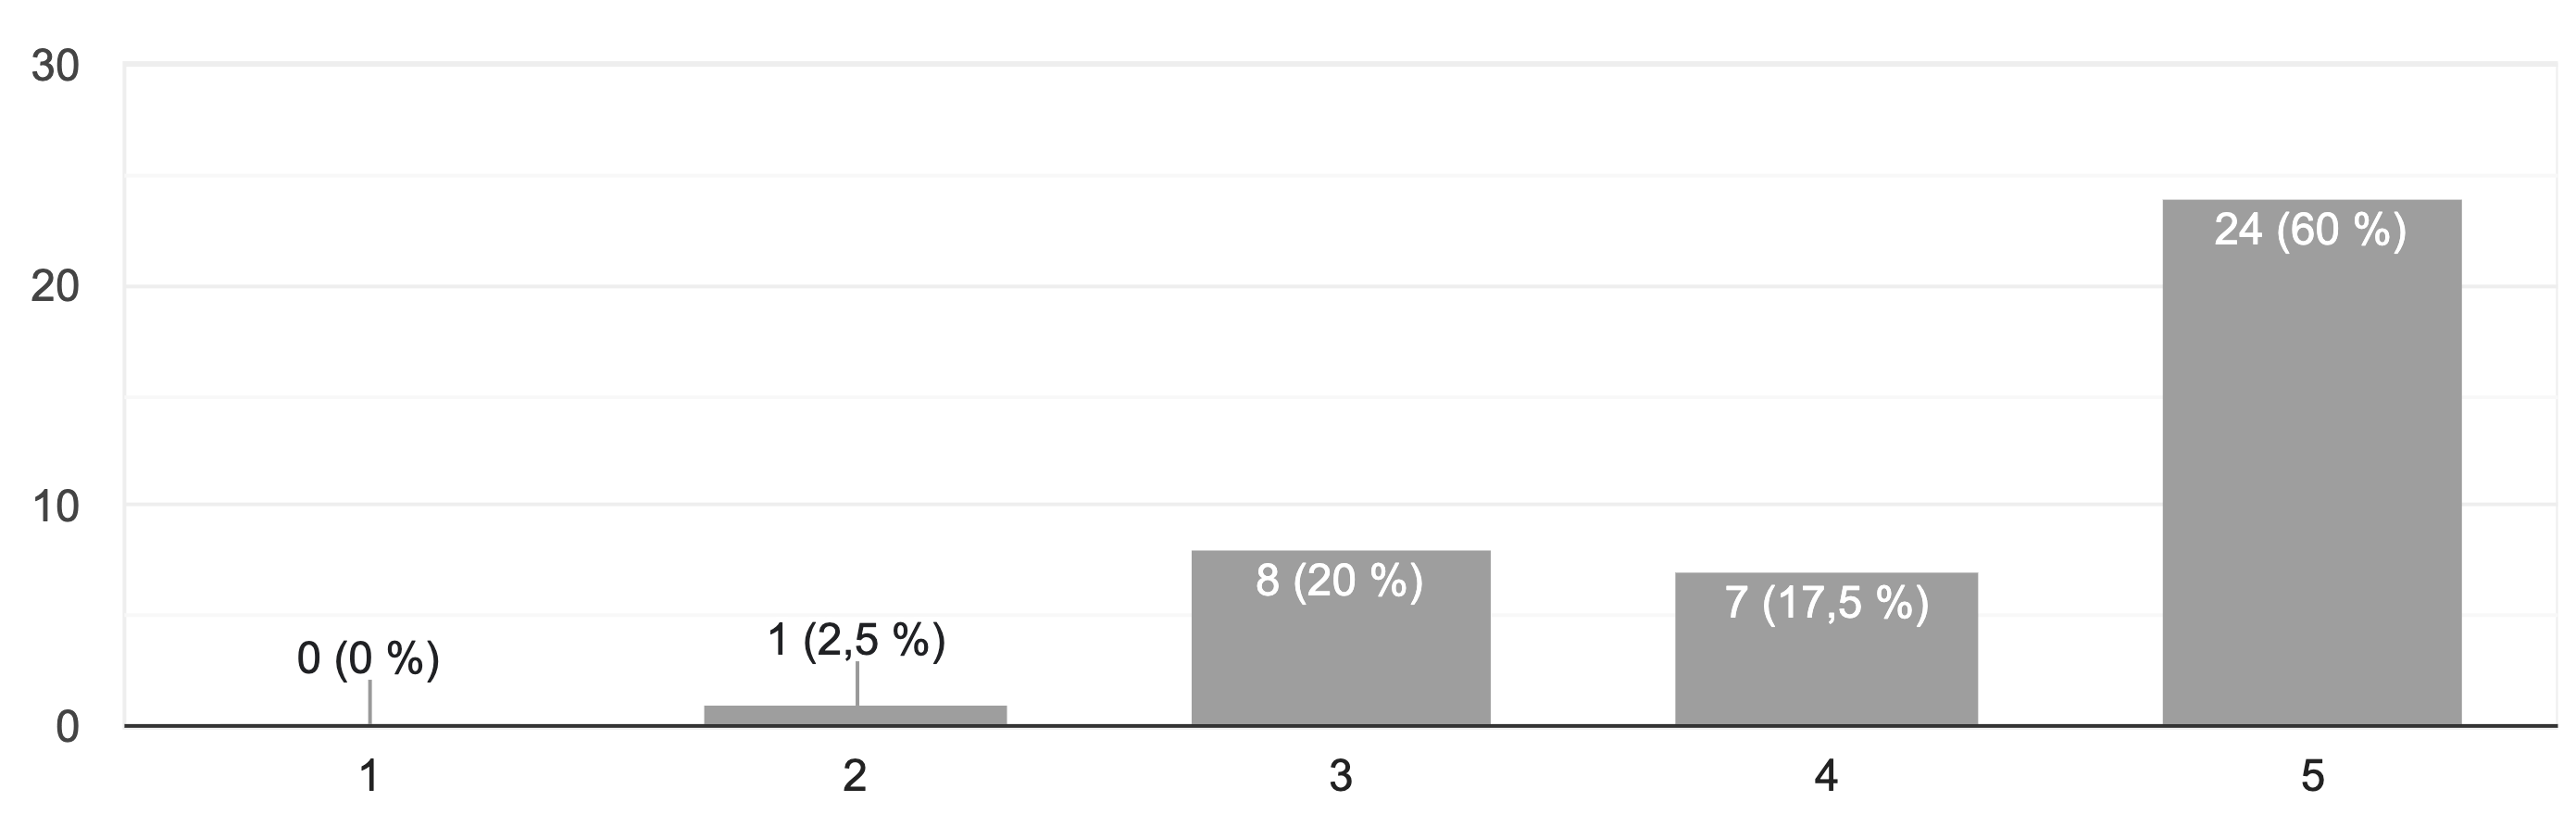
\includegraphics[width=\textwidth]{aufgabe_schwierigkeit_1}
    \caption{Wie schwer fandest du Aufgabe 1? (Auswertung Aufgabe 1)}
    \bildquelle{Google Forms}
    \label{fig:prototyp-umfrage-aufgabe-1-schwierigkeit}
\end{figure}

77,5 \% (31/40) der Befragten gaben an, dass die Aufgabe leicht zu bewältigen war (Schwierigkeitsstufe 4 oder 5). Aufgabe 2 wurde erneut als deutlich schwieriger bewertet. Obwohl 70 \% angaben, dass die Aufgabe leicht zu bewältigen war, lag das Gewicht deutlich mehr auf Schwierigkeit 4 als auf Schwierigkeit 5 (siehe \autoref{fig:prototyp-umfrage-aufgabe-2-schwierigkeit}). Ferner ist der Anstieg bei der Schwierigkeitsstufe 2 (schwer) mit 15 \% signifikant. Bei dieser Einstufung hatte die vorherige Aufgabe im Vergleich nur einen Anteil von 2,5 \% mit einer Stimme. Im Verlauf wird diese Erkenntnis durch eine \autoref{table:prototyp-umfrage-aufgaben-schwierigkeit} mit den stochastischen Werten belegt.

\begin{figure}[H]
    \centering
    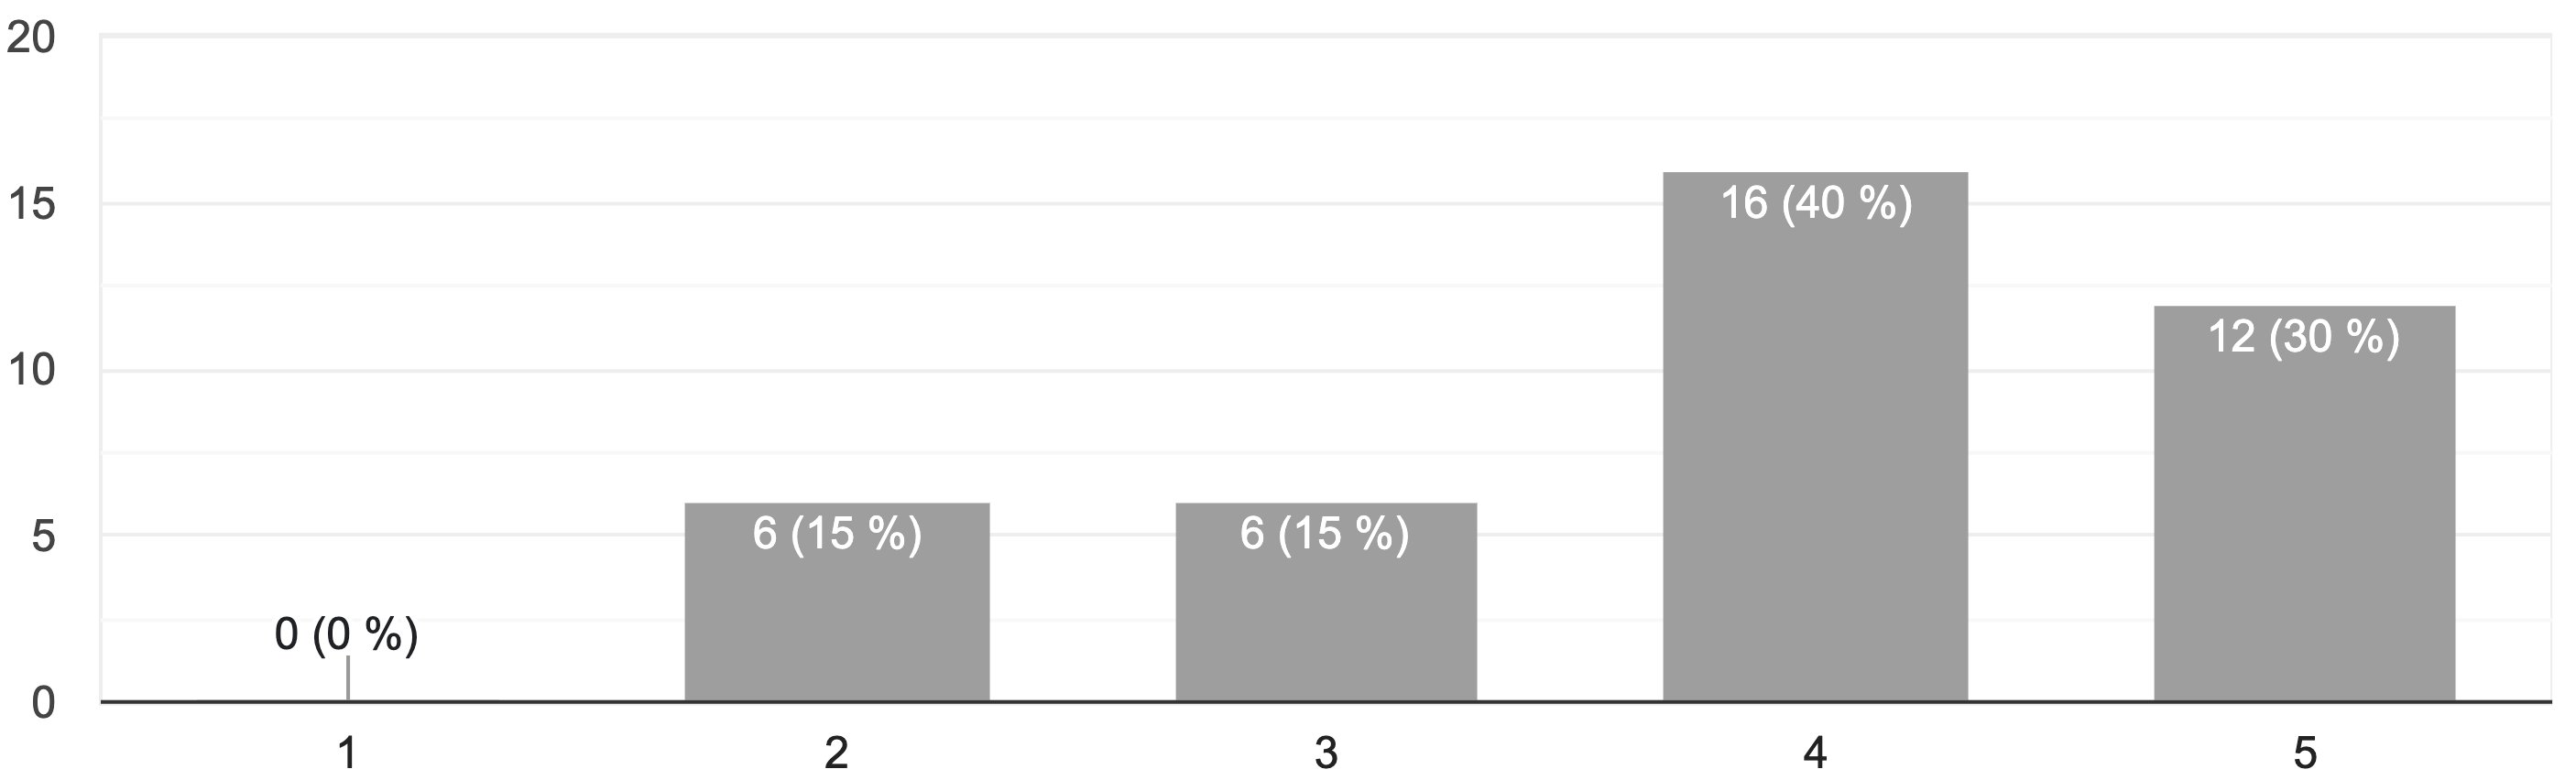
\includegraphics[width=\textwidth]{aufgabe_schwierigkeit_2}
    \caption{Wie schwer fandest du Aufgabe 2? (Auswertung Aufgabe 2)}
    \bildquelle{Google Forms}
    \label{fig:prototyp-umfrage-aufgabe-2-schwierigkeit}
\end{figure}

Zusammenfassend zeigt die stochastische Analyse in \autoref{table:prototyp-umfrage-aufgaben-schwierigkeit} die bereits aus den Diagrammen ersichtlichen Tendenzen. Sowohl der Durchschnitt als auch der Median sind bei Aufgabe 2 niedriger, was darauf hindeutet, dass diese als schwieriger empfunden wurde. Minimum und Maximum sind in beiden Aufgaben gleich. Das bedeutet, dass es bei beiden Aufgaben Befragte gab, die die Aufgaben als sehr leicht und als eher schwer empfanden. Keiner fand die Aufgaben jedoch unlösbar. Die Standardabweichung ist bei Aufgabe 2 höher als bei Aufgabe 1. Dies könnte bedeuten, dass Aufgabe 1 so einfach war, dass es für viele selbstverständlich war, die richtige Lösung zu finden und deshalb der Großteil sehr einfach ankreuzen konnte. Bei Aufgabe 2 lag der Mittelwert eher in der Mitte der Skala, weshalb die Streuung höher ist und somit die Meinungen über die Schwierigkeit stärker differierten. 

\begin{table}[H]
    \renewcommand*{\arraystretch}{1.6}
    \centering
    \begin{tabular}{|l|l|l|l|l|l|} 
    \hline
    \diagbox{\textbf{Fragen}}{\textbf{Ergebnisse}} & \textbf{Durchschnitt} & \textbf{SD} & \textbf{Median} & \textbf{Min.} & \textbf{Max.}  \\ 
    \hline
    \textbf{Wie schwer fandest du Aufgabe 1?} & 4.350 & 0.882 & 5.000 & 2 & 5 \\
    \hline
    \textbf{Wie schwer fandest du Aufgabe 2?} & 3.850 & 1.014 & 4.000 & 2 & 5 \\ 
    \hline
    \end{tabular}

    \caption{Auswertung der Fragen zu den Aufgaben}
    \label{table:prototyp-umfrage-aufgaben-schwierigkeit}
\end{table}

\paragraph{Umfrage Teil 3: Aufgaben}

Der dritte Teil der Studie beinhaltet drei Fragen, die von den Schülerinnen und Schülern in Freitextfeldern beantwortet werden konnten.  Aus diesem Grund werden auch diese Felder mithilfe von Wordclouds ausgewertet. So kann man schnell einen Überblick über die wichtigsten Punkte der Antworten erhalten.

% Was findest du am Konzept gut?

\begin{figure}[H]
    \centering
    
\includegraphics[width=0.6\textwidth]{aufgabe3.1-wordcloud}
    \caption{Wordcloud zu \glqq Was findest du an dem Konzept gut?\grqq{} (Umfrage Teil 3)}
    \bildquelle{Eigene Darstellung}
    \label{fig:prototyp-umfrage-aufgaben-3-1-wordcloud}
\end{figure}

\autoref{fig:prototyp-umfrage-aufgaben-3-1-wordcloud} zeigt die Wordcloud für die erste Frage des letzten Umfrageteils \glqq Was findest du an dem Konzept gut?\grqq{}. Wie bei der vorherigen Wortwolke sind häufig verwendete Begriffe prominenter (größer), während kleinere Begriffe nur selten verwendet wurden. Wie zuvor sind auch hier die vollständigen Antworten im Anhang zu finden. Ignoriert man die Begriffe \textit{Studiengang} und \textit{Studiengänge}, sind die Begriffe \textit{vergleichen} und \textit{Vergleich} mit insgesamt 20 Vorkommnissen sehr präsent. Es lässt sich schlussfolgern, dass die Implementierung der Vergleichsfunktion in den Prototypen erfolgreich ist und weiterverfolgt und optimiert werden sollte.

Weitere Schlagwörter, die ins Auge fallen, sind \textit{schnell}, \textit{übersichtlich}, \textit{Überblick}, \textit{direkt}, \textit{leicht}, \textit{praktisch} und \textit{ähnliche}. Diese Begriffe beziehen sich möglicherweise auf das allgemeine Konzept des Studiengangsfinders und unterstützen erneut die Basis des Konzepts, dass eine solche Art von Software bei der Studiengangsfindung für Studieninteressierte sehr nützlich sein kann.

% Was findest du am Konzept schlecht?

\begin{figure}[H]
    \centering
    
\includegraphics[width=0.6\textwidth]{aufgabe3.2-wordcloud}
    \caption{Wordcloud zu \glqq Was findest du an dem Konzept schlecht?\grqq{} (Umfrage Teil 3)}
    \bildquelle{Eigene Darstellung}
    \label{fig:prototyp-umfrage-aufgaben-3-2-wordcloud}
\end{figure}

Die zweite Frage lautete: \glqq Was findest du am Konzept schlecht?\grqq{} Für diese Frage wurde ebenfalls eine Wordcloud erstellt (siehe \ref{fig:prototyp-umfrage-aufgaben-3-2-wordcloud}). Um alle Punkte vollständig zu erfassen, wurde jedoch hauptsächlich mit den Original-Antworten gearbeitet. Der größte Begriff in Bezug auf die Zufriedenheit war \textit{nichts}, was bedeutet, dass der Großteil mit dem Prototyp bereits zufrieden war. Bei genauerer Betrachtung lassen sich jedoch einige Kritikpunkte feststellen:

\begin{itemize}
    \item Übersichtlichkeit bei vielen Bubbles
    \item Platzierung von Bubbles wirkt willkürlich
    \item Beim Vergleich ist nicht klar erkennbar, welche Farbe dem ursprünglich ausgewählten Studiengang und welche dem Vergleichsstudiengang zugeordnet ist
    \item In der Funktion \glqq Studiengang vergleichen\grqq{} sollten die Studiengänge entweder alphabetisch sortiert oder durch eine Suchfunktion filterbar sein.
    \item Legende für direkten Vergleich einfügen
    \item Die Vergleichsoption sollte auffälliger gestaltet werden
    \item Was passiert, wenn ein Studiengang inhaltlich in zwei übergeordnete Gruppen fällt?
    \item Erforderliche Soft Skill mit angeben
    \item Button \glqq Mehr erfahren\grqq{} geht in der Übersicht unter
    \item Einstiegsgehalt in absoluten Zahlen
\end{itemize}

Zusammenfassend sollte die Platzierung der Bubbles erklärt werden. Diese erfolgt nicht willkürlich, sondern mithilfe des MDS-Algorithmus und der Inhalte des Studiengangs automatisch. Im finalen Produkt werden die Bubbles voraussichtlich durch einen besseren Datensatz auch geschickter platziert, wodurch sich dieser Kritikpunkt vermutlich erledigen sollte.

Die Farbe des Vergleichsfeatures wurde mehrmals kritisiert. Im Moment werden die Inhaltsbalken des zu vergleichenden Studiengangs mit einem neutralen Grau über die des original angeklickten Studiengangs gelegt. Eine mögliche Verbesserung wäre die Verwendung einer Farbänderung, eines zusätzlichen Hilfe-Dialogs oder einer Legende. Um eine schnellere Suche zu ermöglichen, könnten die zu vergleichenden Studiengänge vor der Auslieferung ans Frontend durch das Backend alphabetisch sortiert werden.

Ferner ist es kein Hindernis, wenn ein Studiengang inhaltlich in zwei Gruppen fällt, da immer der höchste Wert zur Gruppenzugehörigkeit gewählt wird. Wenn zwei Kategorien denselben Wert haben und gleichzeitig die höchsten Werte sind, wird die erste Kategorie verwendet. Außerdem ist es kein Problem, da die Wahrscheinlichkeit hoch ist, dass die Bubbles nahe beieinander liegen, wenn der Algorithmus berechnet wird. Selbst wenn sie sich in verschiedenen Supergruppen befinden, werden sie aufgrund ihrer Koordinaten als ähnliche Studiengänge betrachtet.

Es gestaltet sich eher schwierig, erforderliche Soft Skills für das Studium anzugeben, da es keine offizielle Dokumentation über die benötigten Soft Skills pro Studiengang gibt.

Der Button \glqq Mehr erfahren\grqq{} geht in der Übersicht unter. Dieser Punkt wurde nur von einer Person geschrieben und die Schaltfläche ist bereits sehr groß und deutlich sichtbar auf der Seite rechts oben platziert, weshalb dieser Punkt nicht weiter evaluiert wird.

Es wurde zweimal nach dem Einstiegsgehalt in konkreten Zahlen gefragt. Ein Nachteil dieser Implementierung besteht darin, dass die Werte regelmäßig überprüft und gewartet werden müssen, im Gegensatz zur aktuellen Implementierung mit den einfachen Bewertungen \glqq Überdurchschnittlich\grqq{}, \glqq Durchschnittlich\grqq{} usw. Deshalb wird dieser Punkt auch nicht weiter untersucht.

% Hast du neue Ideen für den Prototypen?
% Text: Auch hier muss mit den ganzen Antworten gearbeitet werden
\begin{figure}[H]
    \centering
    
\includegraphics[width=0.6\textwidth]{aufgabe3.3-wordcloud}
    \caption{Wordcloud zu \glqq Hast du neue Ideen für den Prototypen?\grqq{} (Umfrage Teil 3)}
    \bildquelle{Eigene Darstellung}
    \label{fig:prototyp-umfrage-aufgaben-3-3-wordcloud}
\end{figure}

Die in \autoref{fig:prototyp-umfrage-aufgaben-3-3-wordcloud} genannten Punkte ähneln sehr den Kritikpunkten, die in der vorherigen Frage \glqq Was findest du an dem Konzept schlecht?\grqq{} behandelt wurden. Im Folgenden werden die Kritikpunkte auf Basis der Wordcloud und den vollen Antworten der Teilnehmenden gruppiert und zusammengefasst dargestellt. Die Original-Antworten sind, wie bei den vorherigen Fragen auch, im Anhang aufgeführt.


\begin{itemize}
    \item Vergleichsfunktion optisch ansprechender gestalten
    \item Vergleichsfunktion über mehr als zwei Studiengänge
    \item Suchfunktion zur Vergleichsfunktion hinzufügen
    \item Persönlichkeitstest einführen (als Orientierung)
    \item Ähnliche Studiengänge anders platzieren/gestalten
    \item Absolute Werte bei Gehälter
    \item Mehr Informationen zu den einzelnen Fächern ggf. Bezug auf die Schule
    nehmen
    \item Farben ändern
\end{itemize}
%% Punkte einfügen

Die optische Gestaltung der Vergleichsfunktion wurde mehrmals erwähnt. Die Farben und die Gestaltung des Buttons zur Aktivierung der Vergleichsfunktion sowie der Inhaltsbalken sollten geändert werden. Außerdem wurde der Wunsch geäußert, dass man mehr als zwei Studiengänge gleichzeitig vergleichen kann. Es stellt sich jedoch die Frage, ob dies sinnvoll ist, da es auf mobilen Endgeräten schnell unübersichtlich werden könnte. Ein weiterer oft genannter Wunsch ist eine Suchfunktion innerhalb der Vergleichsfunktion. Dies könnte, wie bei der vorherigen Frage bereits beschrieben, entweder durch eine alphabetisch sortierte Liste oder durch ein Autocomplete-Textfeld gelöst werden. Ein Autocomplete-Textfeld schlägt Vorschläge vor, während Buchstaben eingegeben werden. Es ähnelt somit einem Suchfeld.

Außerdem wurde mehrfach ein Persönlichkeitstest gewünscht, der spezifische Fragen an den oder die Studieninteressierte stellt und daraus eine Empfehlung für das zu wählende Studium ableitet. Wie bereits in \autoref{sec:konzepte-von-studiengangsfindern} erwähnt, bringt dies jedoch auch einige Limitierungen mit sich. Eine Möglichkeit für die Zukunft wäre, eine optionale Online-Umfrage anzubieten. Diese könnte die Ergebnisse aufgrund der eingegebenen Daten in StudyMap als eine Art Heatmap darstellen und die Zugehörigkeit zu einer bestimmten Position und somit zu einer Supergruppe bzw. Studiengang markieren. Eine Heatmap ist eine grafische Darstellung von Daten, bei der Werte in einer Matrix durch Farben codiert werden. Intensivere Farben repräsentieren höhere Werte, um Muster oder Trends visuell hervorzuheben. In diesem Fall werden die Zugehörigkeiten zur Kategorie \glqq Wirtschaft\grqq{} dargestellt. 

Es wurde erwähnt, dass die Sektion \glqq Ähnliche Bachelor-Studiengänge\grqq{} nicht gut platziert ist. Dieser Eindruck könnte aufgrund der eher standardmäßigen Gestaltung (siehe \autoref{fig:mockup-bubbles-popup} ganz unten im Popup) entstehen. Eine Möglichkeit wäre, die Studiengänge mit Icons zu versehen oder sie wie bei dem Abschnitt \glqq Firmen in Regensburg\grqq{} mit schwarzen, abgerundeten Rechtecken als Schaltflächen zu präsentieren.

Absolute Werte bei den Gehältern können aus den vorher genannten Gründen nicht umgesetzt werden.

Für die Kurzübersicht wäre es vermutlich zu umfangreich, Informationen zu den einzelnen Fächern bereitzustellen. Das Popup ist bereits sehr voll - mehr Inhalt könnte die Benutzererfahrung negativ beeinflussen. Ein zusätzlicher Reiter für alle Fächer wäre vermutlich zu viel. Um die einzelnen Fächer einzusehen, muss der Interessierte lediglich auf den Button \glqq Mehr erfahren\grqq{} klicken und schließlich den Studienverlaufsplan des jeweiligen Studiengangs öffnen. Dort sind alle präzisen Informationen über den Studiengang für den Benutzer zu finden. StudyMap bietet einen Überblick und eine grobe Orientierungshilfe für das Studium. Für weitere Informationen steht Studieninteressierten die OTH-Website mit detaillierten Informationen zu allen Studiengängen zur Verfügung.

Wie bereits in \autoref{sec:visualisierung-der-studiengänge} erläutert, werden die Bubbles in den Fakultätsfarben eingefärbt. Dies ist eine Anforderung der Vizepräsidentin der OTH-Regensburg und der Fakultäten der Hochschule. Daher kann dem Wunsch nach anderen Farben nicht entsprochen werden. Andere Farben könnten zu Verwirrung führen, da nicht klar ist, warum eine bestimmte Bubble beispielsweise grün gefärbt ist. Die aktuelle Lösung definiert klar, welcher Studiengang welche Farbe erhält. So umfasst z.B. die Supergruppe Technik nicht nur die Studiengänge der Fakultät Maschinenbau, sondern auch die Studiengänge der Fakultät für Elektro- und Informationstechnik. Obwohl die Studiengänge in derselben Supergruppe sind, kann man sie durch die Farben leichter voneinander unterscheiden.

\subsection{Zusammenfassung der Studien}
Zusammenfassend wurde durch die Anwendung der Mockup-Studie ein positiv bewertetes Konzept für den Prototypen entwickelt. Durch den Prozess des User Centered Designs wurden die späteren Benutzer von Anfang an in den Entwicklungsprozess einbezogen. Dadurch wird sichergestellt, dass die Bedürfnisse der Zielgruppe im finalen Produkt möglichst umfassend erfüllt werden.

Da die Anforderungen der Zielgruppe von Anfang an klar definiert sind, kann durch den Einsatz von UCD die Entwicklungszeit deutlich verkürzt werden. Beide Studien erzielten ähnliche Ergebnisse. Der Hauptkritikpunkt an den Entwürfen bzw. dem Prototypen ist die mangelnde Übersichtlichkeit. Zusammenfassend lässt sich festhalten, dass alle Teile des Endprodukts durch Hilfedialoge erläutert werden sollten. Es muss auch geprüft werden, ob eine Legende für die Bubbles als Erklärung erforderlich ist. Der Fokus sollte also auf der Darstellung von möglichst vielen Informationen in möglichst übersichtlicher Form liegen, um den Nutzern einen Überblick und Vergleich aller Studiengänge zu ermöglichen.

Durch die erste Mockup-Studie konnten bereits einige Schwachstellen des Entwurfs behoben werden, die bei der Implementierung des Prototypen berücksichtigt wurden. Bereits in dieser Phase konnte Entwicklungszeit eingespart werden, da Änderungen mithilfe des Mockups vor der ersten Entwicklung geplant werden konnten. Das positive Feedback auf den Prototyp im Rahmen der Prototypenstudie von 37 Studieninteressierten war eine Bestätigung für den Bedarf an StudyMap als Instrument zur Studienorientierung.

Zusammenfassend ist festzuhalten, dass die Studien erfolgreich verlaufen sind. Als Ausblick in die Zukunft könnte ein Orientierungstest interessant sein. Dieser Test würde den Studierenden anhand einiger Fragen eine Position auf der StudyMap zuweisen, damit sie sich die Studiengänge in der Nähe dieser Position genauer ansehen können. Eine weitere Idee für die Zukunft ist, dass mehr als nur zwei Studiengänge inhaltlich miteinander verglichen werden können.
\newpage

% Evaluierung und Validierung
% \section{Evaluierung und Validierung}

\subsection{Beschreibung der Evaluationsmethoden und -kriterien}

\subsection{Durchführung von Tests mit potenziellen Nutzern}

\subsection{Analyse der Ergebnisse aus den Tests}

\subsection{Diskussion der Stärken und Schwächen des Systems}
% \newpage

% Diskussion und Ausblick
\section{Diskussion und Ausblick}

\subsection{Zusammenfassung der Ergebnisse und wichtigsten Erkenntnisse}

\subsection{Vergleich mit ähnlichen Studienorientierungs-Tools}

\subsection{Potenzielle Erweiterungen und zukünftige Anwendungen}
\newpage

% Römische Nummerierung
\newpage
%\pagenumbering{Roman}
%\setcounter{page}{5}

% Literaturliste soll im Inhaltsverzeichnis auftauchen
\newpage
\phantomsection
\addcontentsline{toc}{section}{Quellenverzeichnis}
% Literaturverzeichnis anzeigen
\renewcommand\refname{Quellenverzeichnis}
\printbibliography
% \bibliography{assets/literatur}

% Anhang
\newpage
\phantomsection
\appendix
\section*{Anhang}
\markboth{Anhang}{}
\addcontentsline{toc}{section}{Anhang}
\renewcommand{\thesubsection}{\Alph{subsection}}

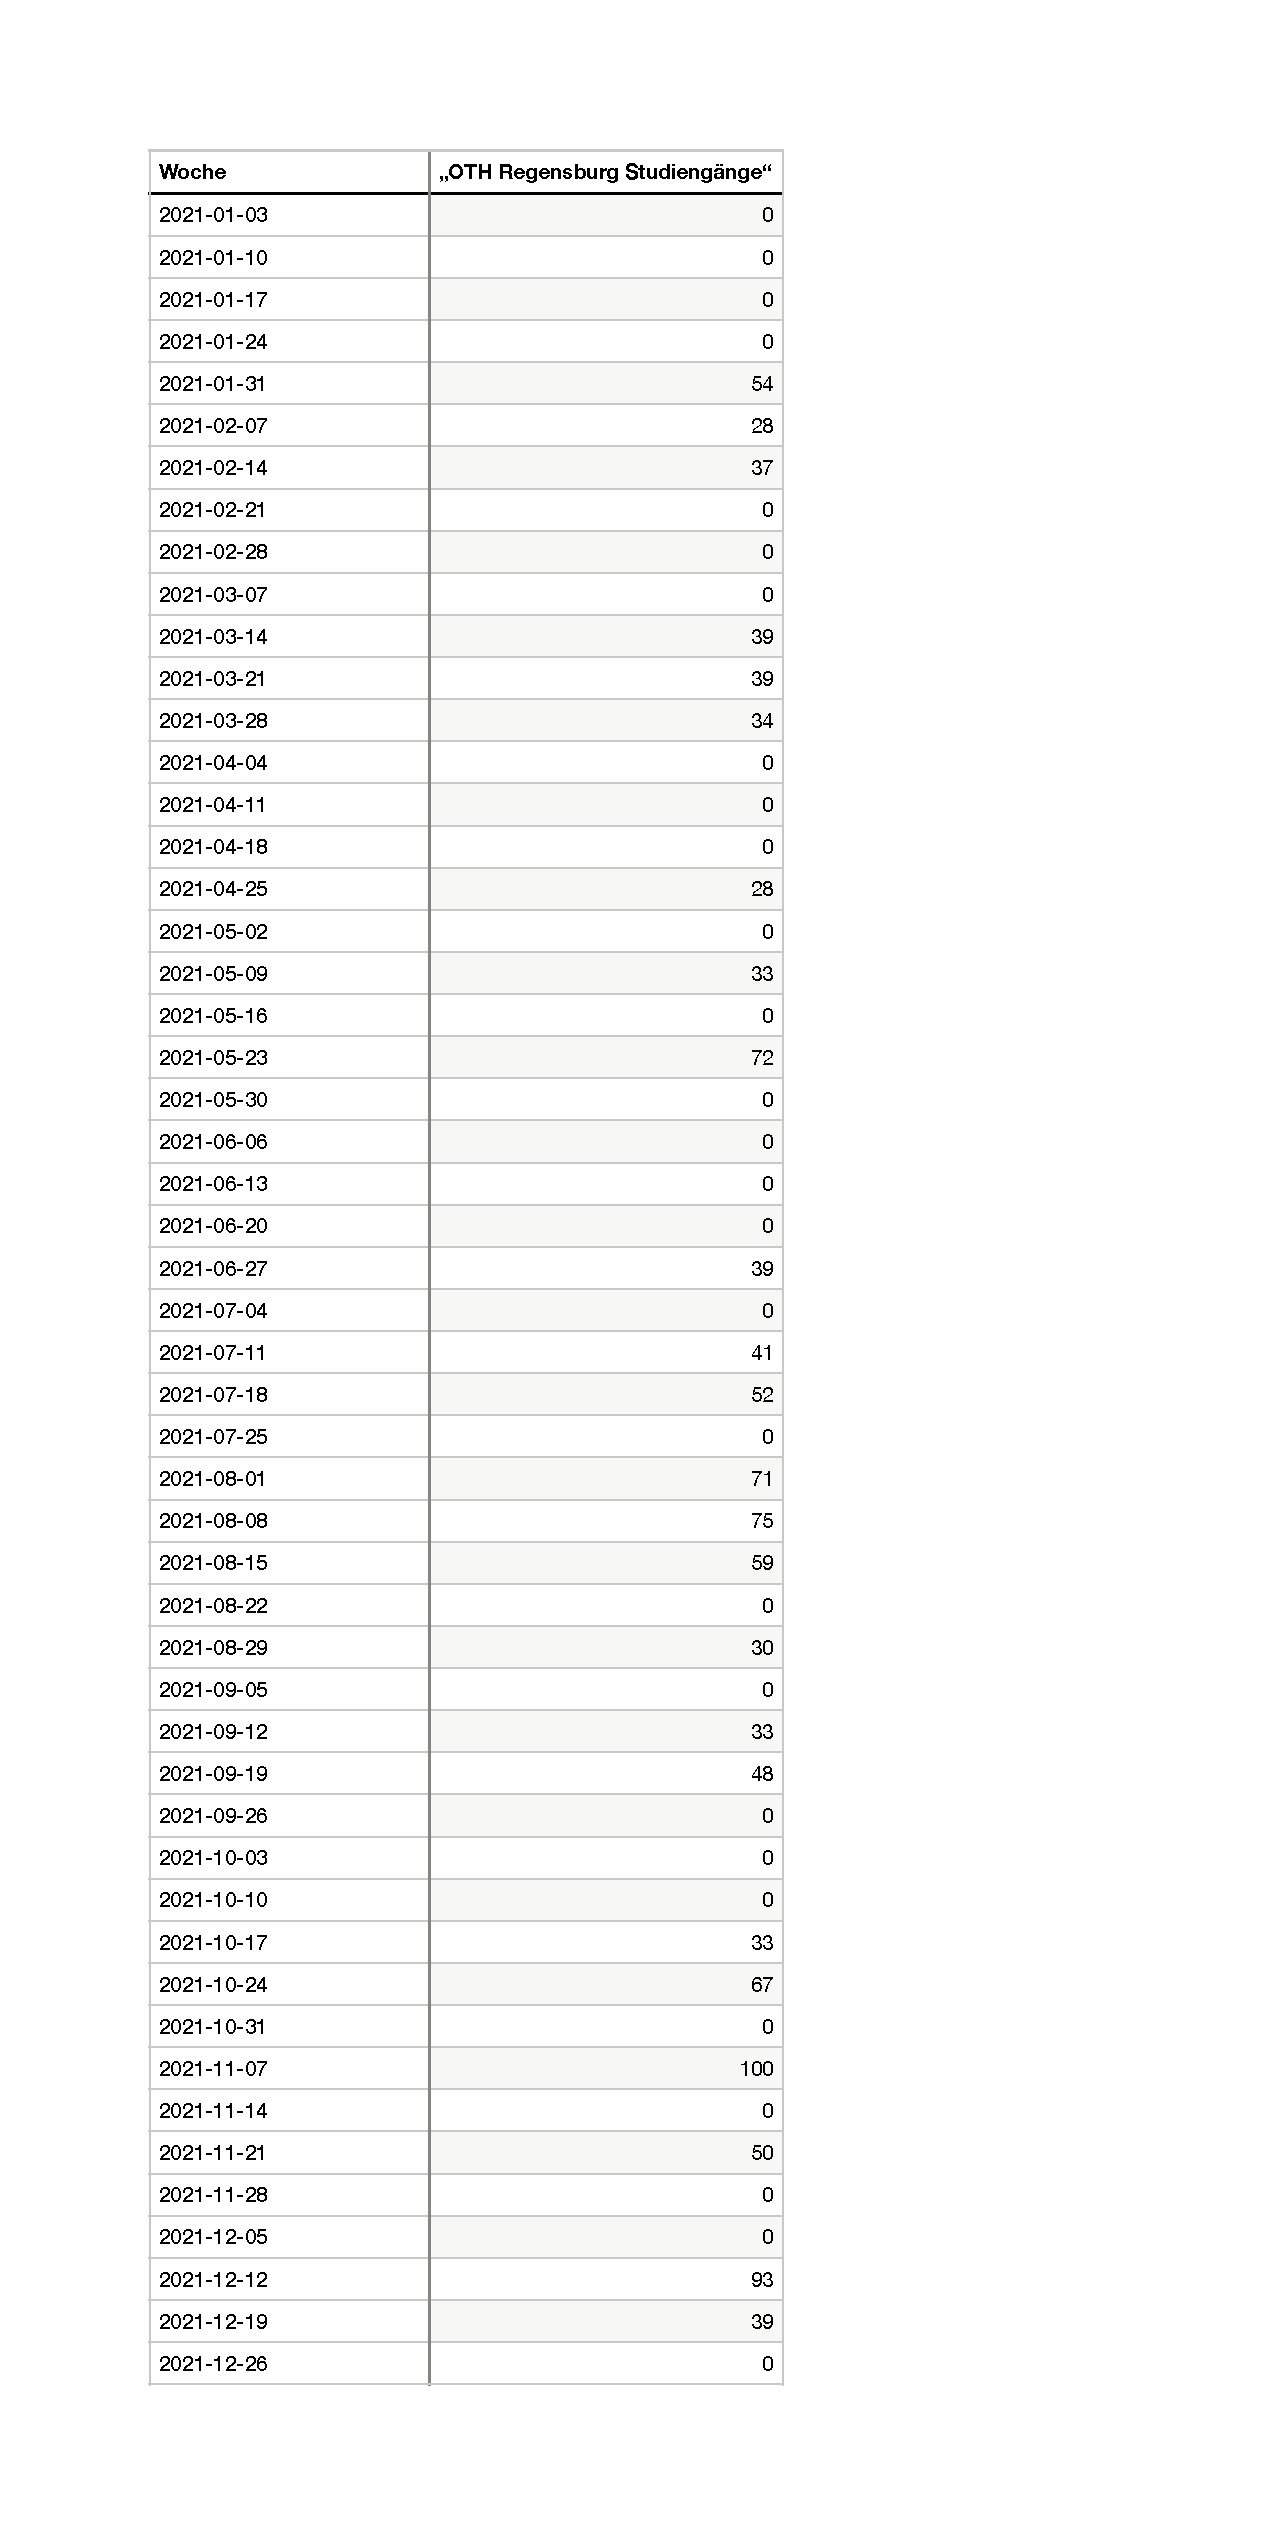
\includepdf[
    clip=0mm 0mm 0mm 0mm,
    trim=0mm 0mm 55mm 0mm,
    pages=1,
    frame,
    scale=.75,
    pagecommand=\subsection{Google Search Trends 2021: \glqq OTH Regensburg Studiengänge\grqq{}}\label{appendix:google-search-trends}
 ]{assets/pdf/google-search-trends.pdf}

\end{document}